\chapter{The CMS L1 Tracking Trigger (CMSL1TT) Project}
\label{app:cmsl1tt}
The CMS Level 1 tracking trigger is a project proposed for the upgrade of the CMS detector during the third stop period of the LHC operation, which is planned to occur around 2020 and goes until around 2025, when should be started the era of the High Luminosity LHC (HL-LHC) Fig.~\ref{fig:lhc_calendar}. 

\begin{figure}[htbp]{16cm}
	\caption{The calendar for the upgrades of the LHC and its detectors.}
	\centering
	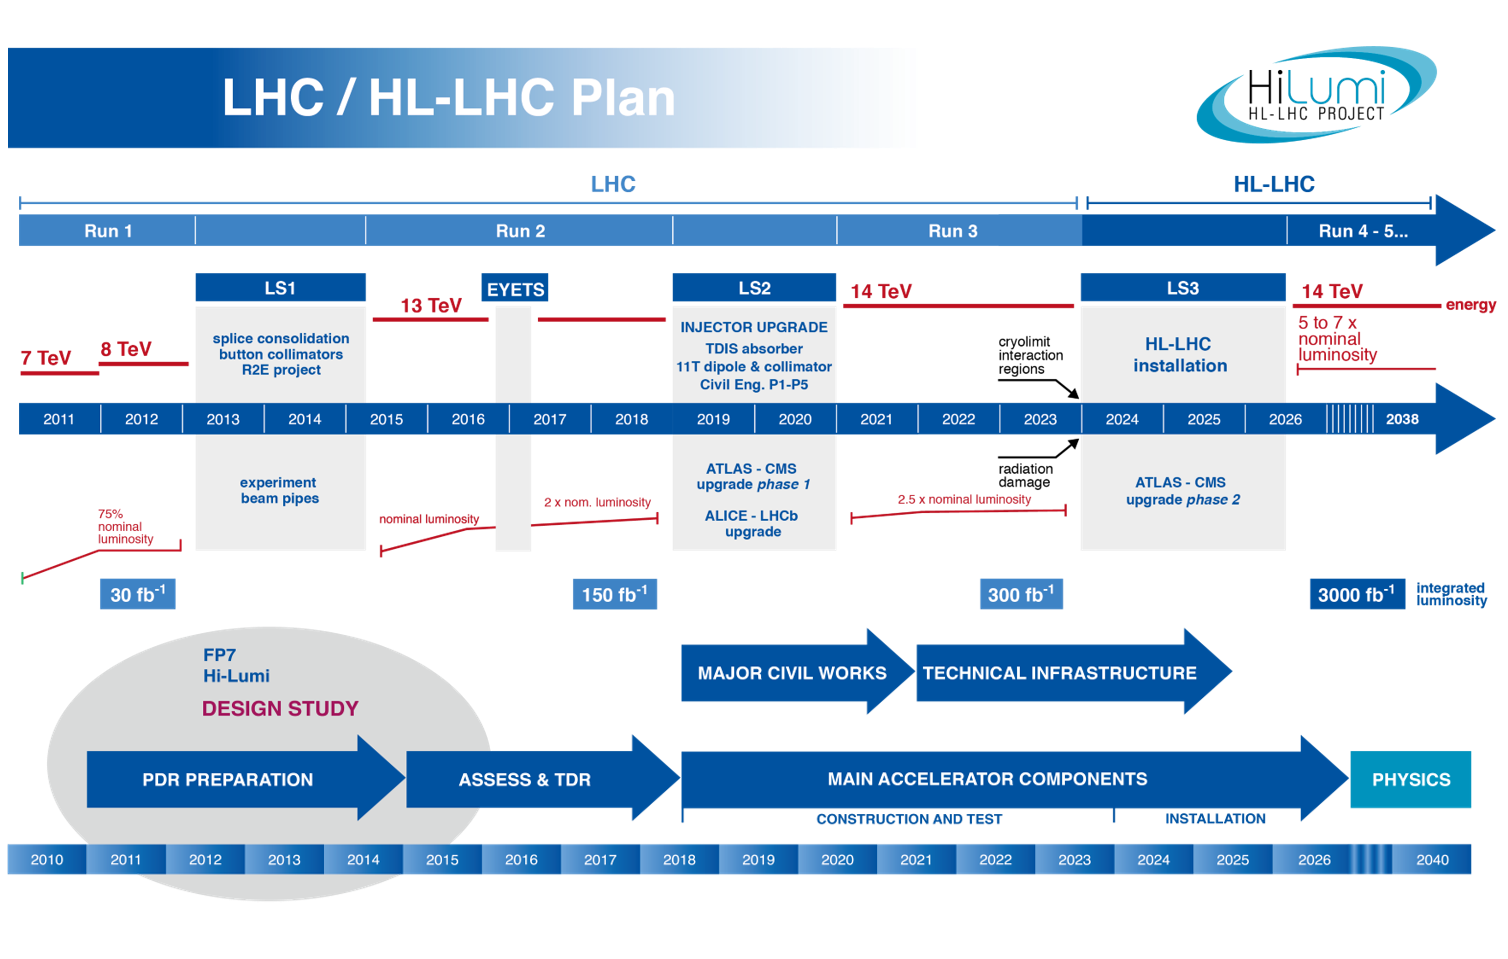
\includegraphics[scale=0.9,angle=90]{AppendixCMSL1TT/figs/Schedule_HLLHC}
	\source{\url{https://project-hl-lhc-industry.web.cern.ch/content/project-schedule}.}
	\label{fig:lhc_calendar}
\end{figure}

In the scenario of the HL-LHC the expected instantaneous luminosity to be provided will be $\sim 10 ^{34} cm^{2}s^{-1}$ (integrated luminosity of 3000fb$^{-1}$) with collisions at the nominal energy at which the LHC was projected, 14TeV. The occurrence of PU has been estimated to be of about 140/200 in average per event \cite{bib:vertex-2017}. Which is a critic condition for the detector operation and for selection of the primary vertices. Since there were some larger PU occurrence (<50> PUs) than the expected one (<30> PUs), the simulation studies also take into account possible extreme scenarios of 250, 300 and 400 PUs. 

The main idea behind the CMSL1TT project is based on the hardware configuration for the phase II upgrade (LS3 in Fig.~\ref{fig:lhc_calendar}). The idea is to include the tracker the information coming from the CMS tracker into the L1 trigger. However, there some significant challenges for such approach. A reasonable estimation of the amount of data given by the tracker is about 600 Gb/s \cite{bib:vertex-2017}. Additionally, the decision returned by the L1 trigger must still be fast (5$\mu s$).

In order to enhance the filtering of PU contribution the hardware of the tracker after phase II will be enhanced. Each tracker layer will be composed of two silicon sensors, back-to-back and interconnected, such that, every time a particle crosses the layer it will produce an object called as \textit{stub}. The stub is a kind of vector which links the centroids of sensor (or cluster of them) in each of the detector layer. Additionally, the distance between those centroids ($SW$ in Eq.~\ref{eq:pt_stub_relation} and $\Delta S$ in Fig.~\ref{fig:stub_definition}), taken orthogonally to the sensors, can be correlated to the $p_{T}$ o the crossing particle. The relation is usually expressed as

\begin{equation}
p_{T} = 0.57 ~ \frac{q . r . \epsilon}{SW . p} ~ \sqrt{1+\frac{sin \theta_{0}}{cos(\theta_{0}-\alpha)}}
\label{eq:pt_stub_relation}
\end{equation}

where, $q$ stands for the charge of the particle, $r$ stands for the average distance of the sensors to the detector coordinates origin (\textbf{xy}), $\epsilon$ stands for the distance between the sensors back-to-back, $\theta_{0}$ is the angle between the particle trajectory and the beam axis and, $p$ is the strip pitch in millimeters \cite{bib:CMS-TDR-17-001}. The Fig.~\ref{fig:stub_definition} shows schematically the idea of the stub. With this approach, it is easy to apply threshold in the $p_{T}$ of the detected particles and remove in a fast way PU particles, which have in average $p_{T} <$ 2GeV. This is the core working principle of the CMSL1TT project.

\begin{figure}[htbp]{16cm}
	\caption{Scheme of the sensors in a layer of the CMS detector after the phase II upgrade. An object called \textit{stub} is defined in terms of the distance between the centroids of back-to-back sensors (or cluster of them) activated when a particle cross the layer.}
	\centering
	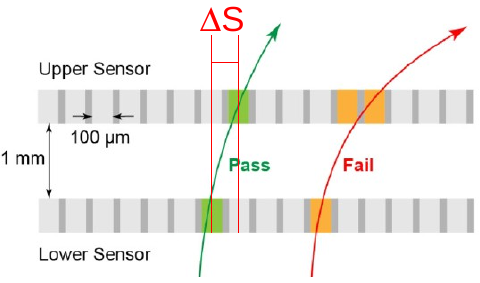
\includegraphics[scale=0.6]{AppendixCMSL1TT/figs/stub_definition}
	\source{Adapted from \cite{bib:CMS-DN-15-025}.}
	\label{fig:stub_definition}
\end{figure}

\section{The Three CMSL1TT Approaches}
At the time the author was cooperating with Fermilab, there were three groups carrying different approaches on how to deal with the track information extraction within the CMSL1TT. These three approaches were: the Associative Memory (AM) + FPGA, the FPGA-based Hough Transform and the FPGA-based Tracklet. As it is clear from their names, the three of the approaches uses FPGAs\footnote{Field Programmable Gate Array (FPGA) is a semicondutor device (a special chip), which can be programmable with routines at hardware level (and not software level) and allows one to create several logic circuits inside just one chip. Different from usual chips, usually called ASIC (Application Specific Integrated Circuits) which are fabricated for specific purposes, the FPGAs can be used for any application. More details see \cite{bib:fpga_xilinx}.}.

The three approaches treat the CMS detector in similar way. In order to properly process the signals coming from the CMS, the detector is divided into small regions called \textit{trigger towers}. Each of these trigger towers are handled separately but using the same idea of the give approach. This first step is usually called \textit{data formatting}. Then, the second step is to find coarse patterns across the hits left by particles in the detector. This step is usually called \textit{pattern recognition} and is here where the three approaches start to go over different paths. The name of the approaches also explains this step for each of them. The AM+FPGA is the one developed by the Fermilab group and the one the author got involved. So, it will be discussed in more details in the next sections. More details about all these approaches can be found in \cite{bib:CMS-TDR-17-001}.


\section{The AM+FPGA CMSL1TT Approach}
The AM+FPGA approach makes the pattern recognition by using the so called Associative Memory. This method runs a parallel matching of the hits found in the detector and the hits found in simulated patterns. This patterns are the so called \textit{roads}, which are coarse track patterns. These roads are composed by what have been called in this approach as \textit{super-strips}, which are the cluster of activated silicon strips in detector layers. Fig.~\ref{fig:pattern_match} illustrates these nomenclatures. Once the number of fired super-strips is achieved for a given pattern, that pattern is triggered and the hits observed in the detector are saved for a most robust fit in order to extract the adequate track properties.

\begin{figure}[htbp]{16cm}
	\caption{Scheme of the partition adopted in the CMSL1TT AM+FPGA for the cluster of strips activated in the silicon sensors in the detector layers.}
	\centering
	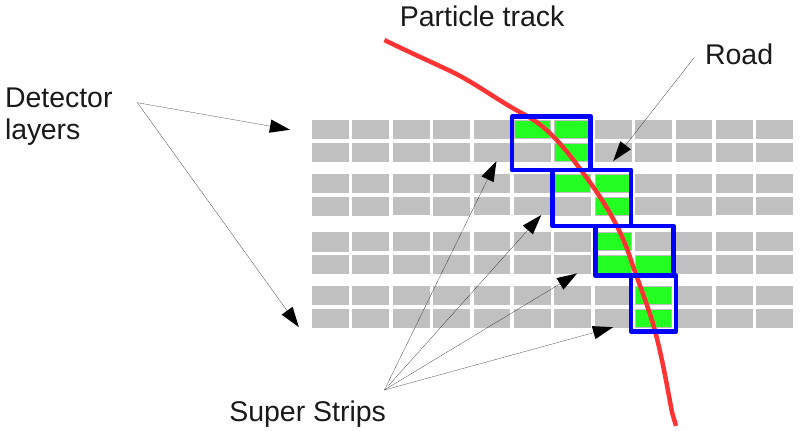
\includegraphics[scale=0.4]{AppendixCMSL1TT/figs/road_example}
	\label{fig:pattern_match}
\source{The AUTHOR, 2016.}
\end{figure}

After the pattern recognition step, the triggered hits coming from the detector are given to a module called \textit{combination builder}, which builds up all the possible tracks by combining those hits. The combinations are then given to another module, called \textit{track fitter}, which performs a fit based on a linearized $\chi^{2}$. In this step one gets the tracks with good resolution parameters. To enhance the selection of tracks and random combination that still looks like a good track, it was developed the procedure called \textit{duplicate removal} (which will be discussed in the following sections). Finally, the tracks that pass the duplicate removal steps are the ones that should be give ot the L1 trigger.

In the following sections the work developed by the author inside the CMSL1TT AM+FPGA approach is presented. For full details, refer to the author presentations (\cite{bib:miqueias-cmsl1tt-19-01-16,bib:miqueias-cmsl1tt-14-04-16,bib:miqueias-cmsl1tt-19-04-16,bib:miqueias-cmsl1tt-27-04-17,bib:miqueias-cmsl1tt-17-08-17}) about these studies.


\subsection{The Simulation Studies for the CMSL1TT AM+FPGA}
In the simulation side, a couple of studies and implementations have been done through the AM simulation package maintained by Fermilab, Florida and TAMU working groups \cite{bib:cmsl1tt_fnal_package}. In the next sections, each study will be described in separated sections and full relevant details about them will be shown. Such studies comprehend synthetic efficiency, duplicate removal, stub bending, roads and combinations truncation, road sorting effect under truncation and track fitter $\chi^{2}$. Synthetic efficiency is designed to quantify track reconstruction efficiency based on track parameters, which can be linked to the analytic efficiency (based on stubs) as will be presented here. Once the AM + FPGA approach produces replicated tracks a duplicate removal (DR) method is needed in order to mitigate those redundant tracks. The stub bending information ($\Delta S $) was used to reduce the number of roads and combinations coming out from AM in order to reduce processing time latency and reduce truncation effects (being very important for busy environment cases such $\mu + PU200$). Good results were achieved using DR and $\Delta S$, keeping track reconstruction efficiency in an acceptable level. Also, when truncation is applied the road ordering has significant impact on the pattern match efficiency. The results presented here were obtained over different event samples which were: ($\mu$/$\pi$/$e$) + PU(140,200,300,400), $\nu$ + PU(140, 200, 250), $t\bar{t}$ + PU200 and jet($p_{T}=250GeV$) + PU200. Jet sample had 2k events and all the others had 10k.

\subsubsection{Roads and Combinations Truncation}
Some of the results presented in these notes concern to simulations in which truncation on roads and combinations was applied. The standard truncation limits were 200 roads and 500 combinations. In order to make the truncation easily modifiable in case of need, one extra flag was implemented in the AM package. The flag for road truncation is \textbf{$--$maxRoads} (implemented on \textbf{PatternMatcher.cc} and \textbf{TrackFitter.cc} modules) and it can act either during the pattern recognition (pattern match) or tracking fitting stage. The combination truncation were previously implemented to truncate combinations per road but, the adequate one is a truncation in combinations per event. For that, the flag \textbf{$--$maxCombsPreCB} was implemented. It works only in the track fitting stage and it essentially counts how many simple combinations are being generated in a given event. Simple combination means that, for each road the number of combinations is the product of the number of stubs per layer. Note that, the advanced combination builder builds extra combinations from 6/6 and it was decided to not account them for the truncation. By default, no road or combination truncation is active in the package (user must specify the truncation limits in the command line).


\subsubsection{Road Sorting Effects under Truncation}
Truncation is a latency holder that needs to be carried out carefully. When truncation is applied it might throw away things it should not. One thing that can affect that is how the list of roads and combinations are handled in AM processing stages. A study was made to verify how the road sorting affect the road efficiency when truncation is applied. Fig.~\ref{fig:road_sorting} shows that for three road sorting ways in $t\bar{t}+PU200$ events: based on pattern $p_{T}$, based on pattern frequency and randomly sorted. The random sort is not straightforward to interpret since it depends on how the randomization sits the roads in the list. In order to get a more precise result it was done a sampling for each sf config. The points in Fig.~\ref{fig:road_sorting} for random sorting are the average from those runs. No big variation was seen (max of 0.003 for sf0.8). It was pointed that sorting the roads by frequency is the better way and that is confirmed by the plot. In the AM package the roads come out from the pattern match stage naturally already sorted by frequency, so no need to implement something new for that. It was also decided to remove any sorting after the pattern recognition stage (since that is not straightforward to have on hardware). Then, no track sorting by decreasing $p_{T}$ after the tracking fit stage was used. Also, in DR the track sorting based on increasing track fitter $\chi^{2}$ was removed.

\begin{figure}[htbp]{15cm}
	\caption{Road sorting effect on efficiency without truncation and with truncation in 200 roads and 500 combinations for $t\bar{t}+PU200$.}
	\centering
	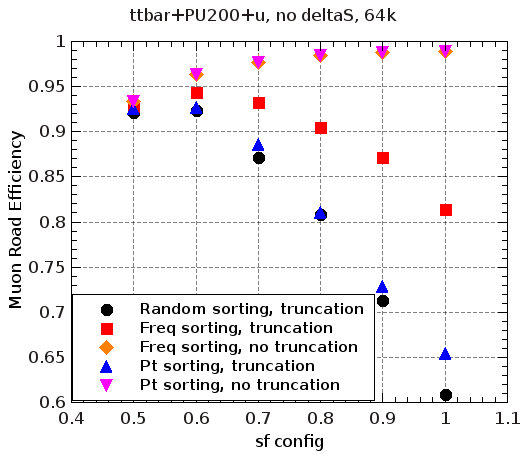
\includegraphics[scale=0.6]{AppendixCMSL1TT/figs/ttbar_pu200_mu_road_sorting_comparison}
	\label{fig:road_sorting}	
\source{The AUTHOR, 2016.}
\end{figure}


\subsubsection{Stub Bending ($\Delta S$) \label{sec:stub_bending_approach}}
The stub bending is one of the core concepts of CMS L1TT being the main variable projected to allow fast cut on low $p_{T}$ tracks such as the ones coming from pile up. Stub bending is a measurement of the distance between cluster centroids of correlated silicon sensors in each of the detector layers. That distance is measured in terms of half silicon strip. A study was developed in order to investigate the usage of stub bending information as a way to avoid random pattern firing. That is, without $\Delta S$ an AM pattern is fired by random tracks that can cross the layers in very different angles. Looking at the $\Delta S$'s of combinations produced by such random tracks one can see that they are incompatible as sketched in Fig.~\ref{fig:deltaS_workway}. Now, if the stub bending can be used to build up AM pattern banks (such as with \textbf{$\phi$} or \textbf{z} segmentation) than those random tracks will not fire a pattern anymore.

\begin{figure}[htbp]{15cm}
	\caption{How the $\Delta S$ mitigate AM patterns fired by random tracks: two random tracks trigger a valid pattern and the stubs are stored for further analysis but, the stubs combination doesn't come from a real track.}
	\centering
	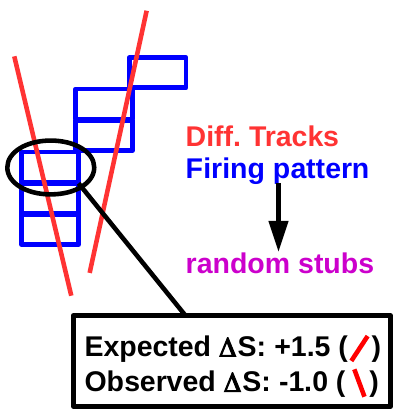
\includegraphics[width=5cm,height=5cm]{AppendixCMSL1TT/figs/deltaS_workway}
	\label{fig:deltaS_workway}
\source{The AUTHOR, 2016.}
\end{figure}

The $\Delta S$ encoding to create AM pattern banks was done by dividing the stub bending distribution in ranges. Each range then is identified by an integer index which one is used to define the superstrips ID (ss ID). Once the standard configuration adopted at that time was $sf1\_nz1$, which means no \textbf{z} segmentation, the same formula to build the ss ID on that case was used, with the change of the \textbf{z} segment index by the stub bending index. The formula, present on module \textbf{SuperstripArbiter.cc}, is the following

\begin{equation}
ss = i_{\Delta S}*N_{\phi} + i_{\phi}
\end{equation}

in which $i_{\Delta S}$ is the stub bending index associated to the range from which a stub belongs, $N_{\phi}$ is the number of $\phi$ segmentations (which depends on the stub fountain scale factor configuration - sf) and $i_{\phi}$ is the $\phi$ segment index associated to the stub. As one can see in Fig.~\ref{fig:deltaS_ttbar_asym} the $\Delta S$ distributions in all layers are centered in zero. The stub bending index is defined from there, that is, the region close to $\Delta S = 0$ is the central range. Then, one can divide the stub bending distribution in many different range sizes. Also, one can try to use ranges with different widths. 

\begin{figure}[htbp]{15cm}
	\caption{Stub bending distribution per detector layer for $t\bar{t}+PU200$ and the $\Delta S$ ranges for the configuration ASYM115577. In the ASYM mode only the central range can have width defined by user and $\Delta S$ always is divided only into 3 ranges.}
	\centering
	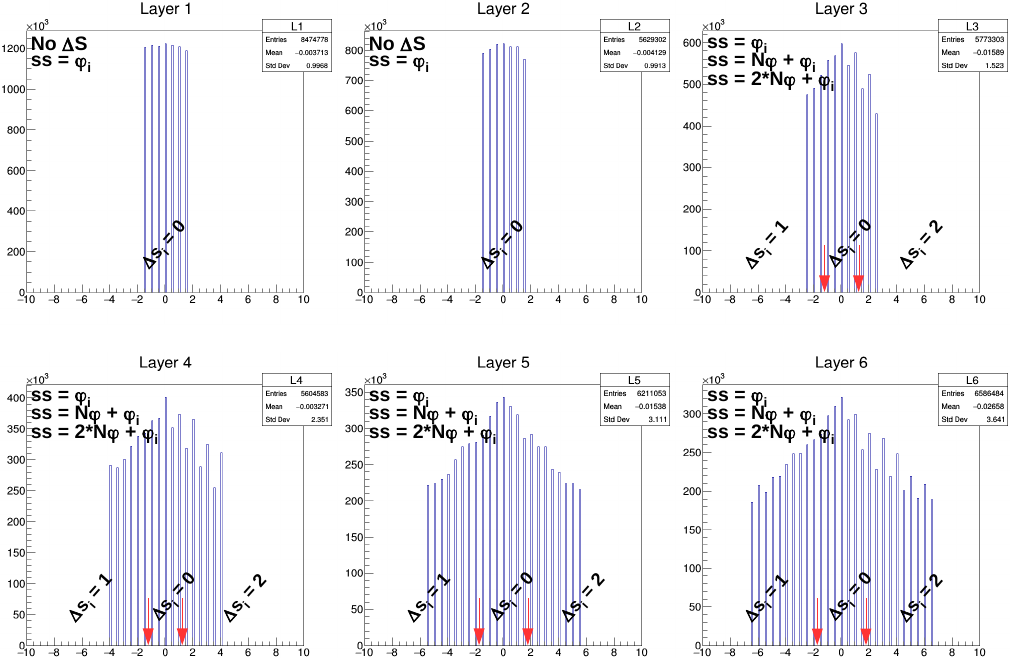
\includegraphics[scale=0.8,angle=90]{AppendixCMSL1TT/figs/ttbar_pu200_asym115577}
	\label{fig:deltaS_ttbar_asym}
\source{The AUTHOR, 2016.}
\end{figure}

\begin{figure}[htbp]{15cm}
	\caption{Stub bending distribution per detector layer for $t\bar{t}+PU200$ and the $\Delta S$ ranges for the configuration SYM115577. In the SYM mode ranges have the same width, except the outer ranges (those ones comprehending $|\Delta S|$ = 6.5).}
	\centering
	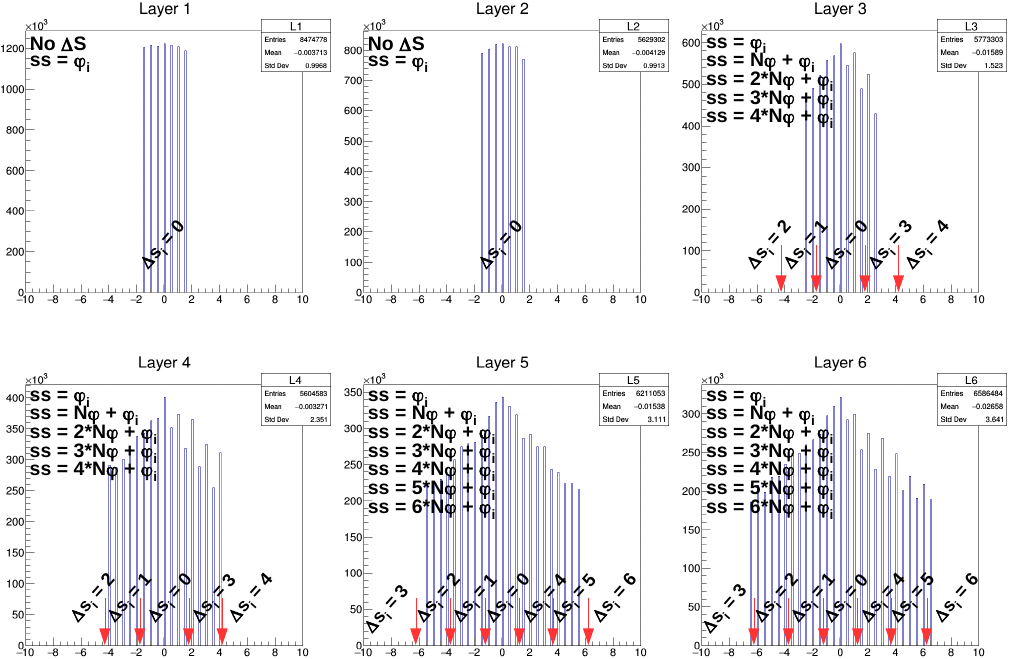
\includegraphics[scale=0.8,angle=90]{AppendixCMSL1TT/figs/ttbar_pu200_sym115577}
	\label{fig:deltaS_ttbar_sym}
\source{The AUTHOR, 2016.}
\end{figure}

On those studies two approaches were developed: one called asymmetric (ASYM) and one called symmetric (SYM). They have completely different structures but show similar performance. In the ASYM the $\Delta S$ distribution is divided always in three ranges and only the central range can have the width adjusted. The SYM was meant to produce all ranges with equal width, being possible to specify how many ranges should be produced. In the AM package that is controlled by two flags: \textbf{$--$deltaSM} that receives a string identifying the approach to be used (ASYM or SYM) and \textbf{$--$deltaS} that receives an integer number of 6 digits that specifies the configuration in each layer. So, for instance, ASYM115577 means that in the first two inner detector layers $\Delta S$ is not divided (that is, the standard way, no stub bending usage), in the two middle layers a central range with 5 $\Delta S$ values is created and in the two outer layers a central range with 7 values. For a configuration like SYM115577, the two inner layer again will not receive any operation, then the two middle layer will contain 5 ranges and the two outer layers will have 7 ranges. In order to calculate how to divide those distributions it was considered the maximum $\Delta S$ absolute value observed. It was found to be the same for $t\bar{t}+PU200$ and $jet(p_{T}=250GeV)+PU200$ (distribution on Fig.~\ref{fig:deltaS_jet250_pu200}), and is equal to 6.5. The division then was previously computed, producing the Tab.~\ref{tab:deltaS_divisions} which was encoded on \textbf{SuperstripArbiter.cc} module. An important note here: the flags specifying $\Delta S$ configuration must be used when generating pattern bank and when doing the pattern recognition step. In tracking fit stage it doesn't play any function since the ss are not used but instead the stubs properties. Also, the maximum value allowed to specify the range width or the number of ranges is 9. Additionally, the numbers must be always odd (since there's the $\Delta S = 0$ value). Any other attempt will produce an error message showing the allowed configurations.

\begin{figure}[htbp]{15cm}
	\caption{Stub bending distribution for $jet(p_{T}=250GeV)+PU200$. Different events seems to have the same limits but, as one can see the occupancy is no equal (comparing with the pictures for $t\bar{t}+PU200$).}
	\centering
	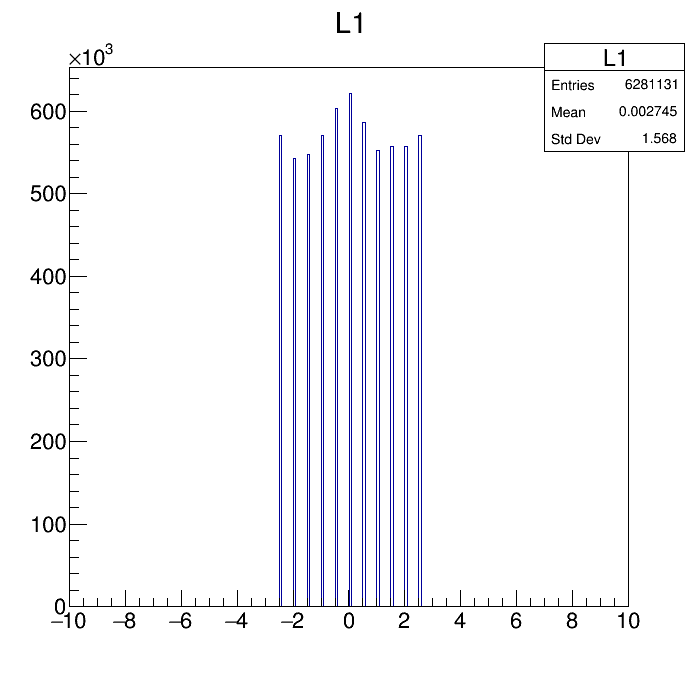
\includegraphics[scale=0.19]{AppendixCMSL1TT/figs/JetPt250_PU200_deltaS_l1}
	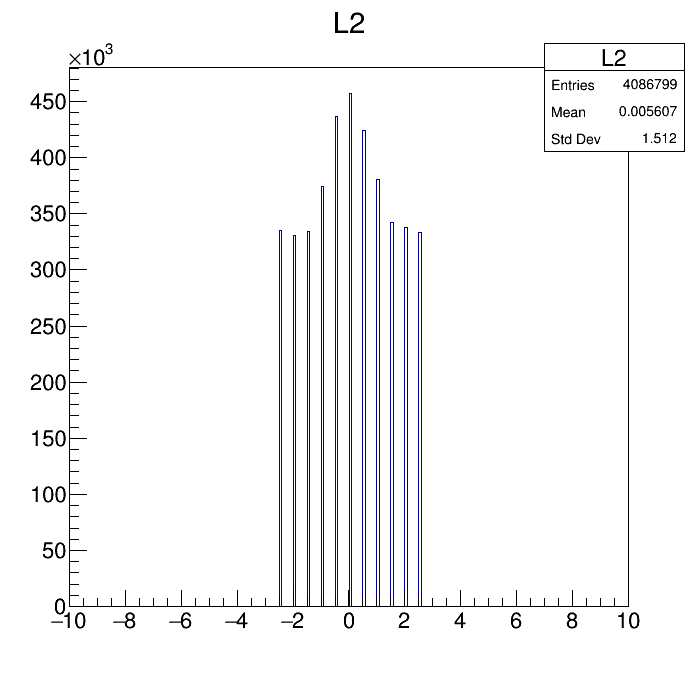
\includegraphics[scale=0.19]{AppendixCMSL1TT/figs/JetPt250_PU200_deltaS_l2}
	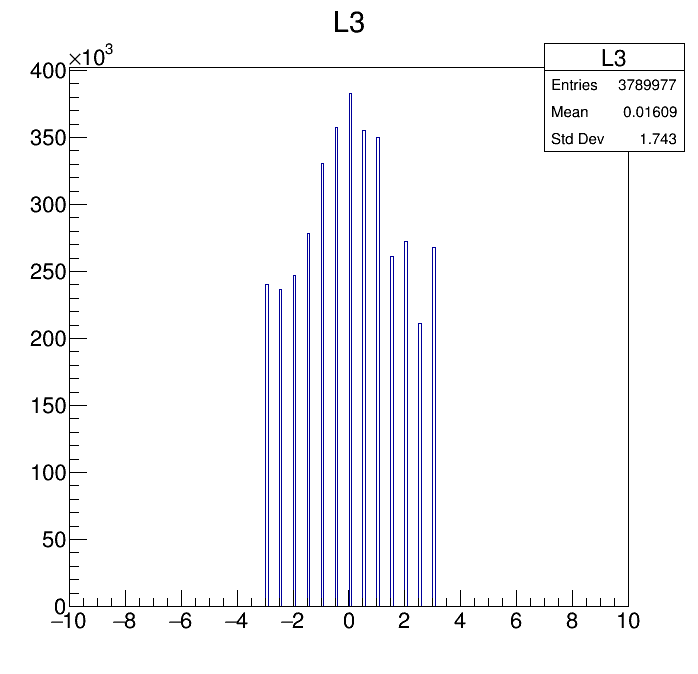
\includegraphics[scale=0.19]{AppendixCMSL1TT/figs/JetPt250_PU200_deltaS_l3}
	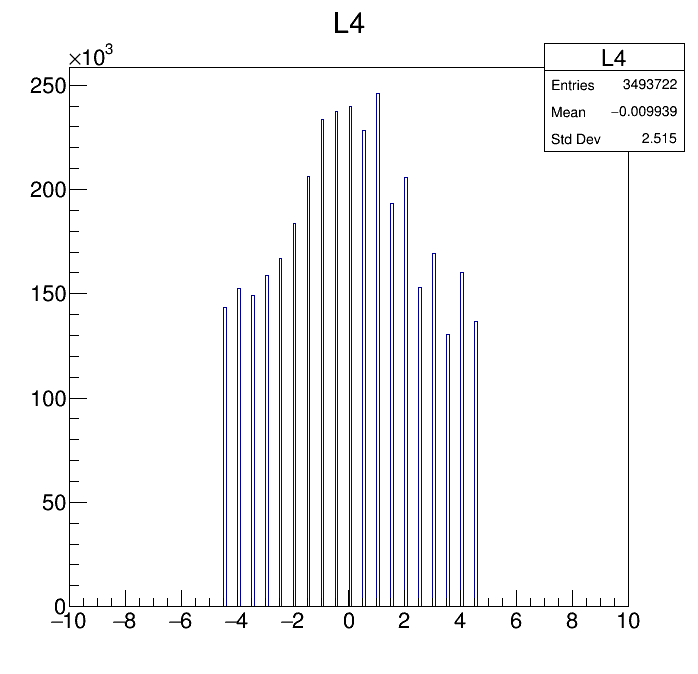
\includegraphics[scale=0.19]{AppendixCMSL1TT/figs/JetPt250_PU200_deltaS_l4}
	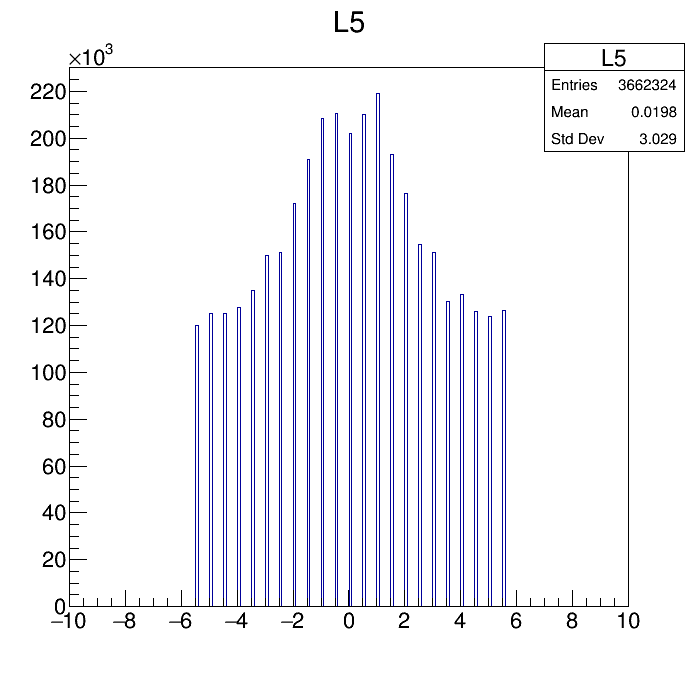
\includegraphics[scale=0.19]{AppendixCMSL1TT/figs/JetPt250_PU200_deltaS_l5}
	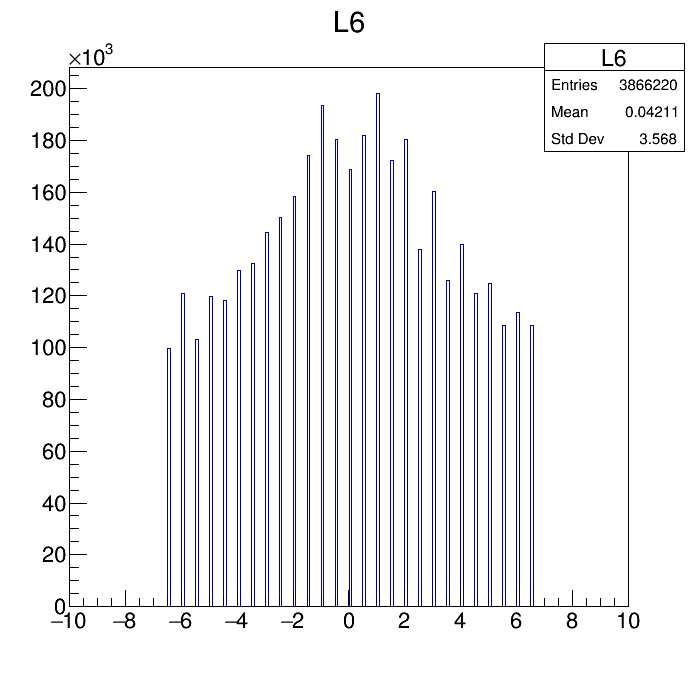
\includegraphics[scale=0.19]{AppendixCMSL1TT/figs/JetPt250_PU200_deltaS_l6}				
	\label{fig:deltaS_jet250_pu200}
\source{The AUTHOR, 2016.}
\end{figure}

\begin{table}[htbp]{15cm}
	\caption{Stub bending possible divisions. The SYM method uses such table to decide how to split the $\Delta S$ values based on the number of ranges requested by user. The negative related of the ranges were omitted in the table.}
	\centering
	\begin{tabular}{c|c|l}
		\hline
		\hline
		$\#$ranges & range width & $\Delta S$ values ({\color{red}[~]} central ranges)\\
		\hline
		3 & 9 & {\color{red}[}-2.0, 2.0{\color{red}]}, [2.5, ...]\\
		5 & 7 & {\color{red}[}-1.5, 1.5{\color{red}]}, [2.0, 5.5], [6.0, ...]\\
		7 & 5 & {\color{red}[}-1.0, 1.0{\color{red}]}, [1.5, 3.5], [4.0, 6.0], [6.5, ...]\\
		9 & 3 & {\color{red}[}-0.5, 0.5{\color{red}]}, [1.0, 2.0], [2.5, 3.5], [4.0, 5.0], [5.5, ...]\\
		\hline 
	\end{tabular}
	\label{tab:deltaS_divisions}
\source{The AUTHOR, 2016.}
\end{table}

Using such implementation many configurations were studied for $sf1\_nz1$. Fig.~\ref{fig:deltaS_roads_combs} shows all tested configurations in comparison with the standard case when $\Delta S$ is not used for $t\bar{t}+PU200$ and for $jet(p_{T}=250GeV)+PU200$. There are three noticeable points on those plots. First, the stub bending is a strong approach to mitigate the proliferation of roads and combinations. In average the reduction factor is about up to 10x for roads and 25x for combinations. Second, there's no big difference on the performances from ASYM and SYM approaches (except for 335577 configuration). Third, $\Delta S$ segmentation in detector inner layers has less effect than in the outer layers. That can be noticed by comparing the black circles, for instance. They represent the combinations $@95\%$. The reduction from standard $sf1\_nz1$ to ASYM115577 is about 90$\%$. Then for ASYM335577 the extra reduction is just about 6$\%$.

The next quantity to look on was the efficiency. In order to avoid the effects from other AM processing stages as tracking fit and DR, it was used the analytic efficiency from roads. Also, it was applied the standard truncation of 200 roads and 500 combinations. As showed in Fig.~\ref{fig:deltaS_trunc_eff} the stub bending has an important role when truncation is applied and the effect is even more significant in jet case. In the better situation it's possible to recover 14$\%$ and 50$\%$ of efficiency for $t\bar{t}+PU200$ and $jet(p_{T}=250GeV)+PU200$, respectively. It's noticeable that for $t\bar{t}+PU200$ the efficiency without and with truncation match for the two last stub bending configurations. Also, one can see that the difference between the ASYM and SYM approaches are more evident in terms of the efficiency. Based on Fig.~\ref{fig:deltaS_roads_combs} and Fig.~\ref{fig:deltaS_trunc_eff}, it was decided that the configuration ASYM335577 is, simultaneously for $t\bar{t}$ and $jets$, the best one.

\begin{figure}[htbp]{15cm}
	\caption{Roads and combinations average and 95 percentile per event versus different $\Delta S$ configurations at $sf1\_nz1$ for $t\bar{t}+PU200$ (left) and $jet(p_{T}=250GeV)+PU200$ (right).}
	\centering
	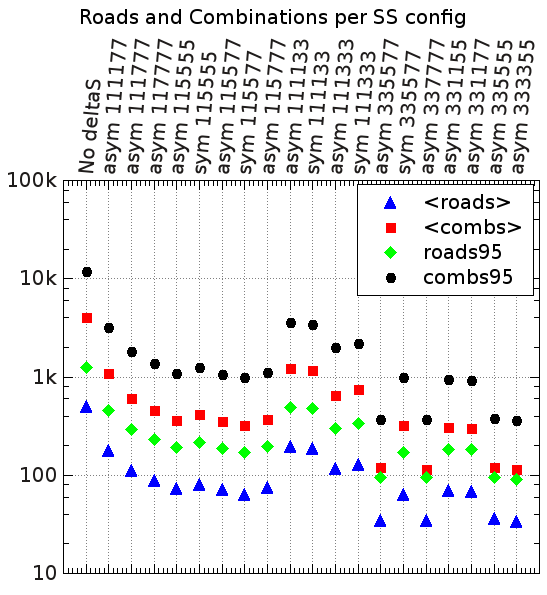
\includegraphics[width=7cm,height=8cm]{AppendixCMSL1TT/figs/final_plots/ttbar_pu200_smu_roads_combs_deltaS}
	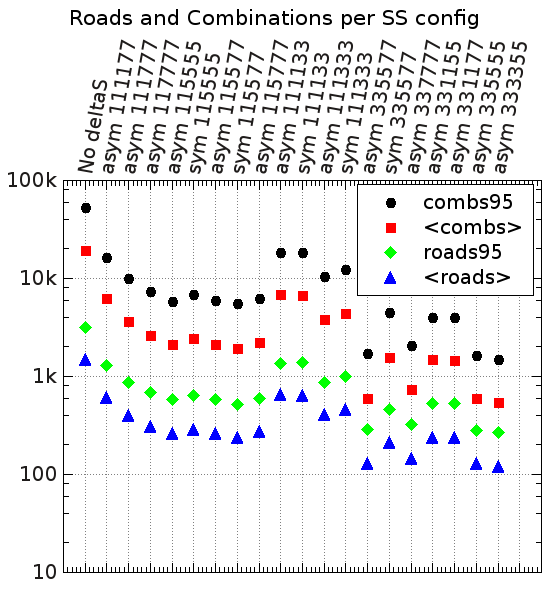
\includegraphics[width=7cm,height=8cm]{AppendixCMSL1TT/figs/final_plots/jet_Pt250_pu200_roads_combs_deltaS}
	\label{fig:deltaS_roads_combs}
\source{The AUTHOR, 2016.}
\end{figure}

\begin{figure}[htbp]{15cm}
	\caption{Road efficiency versus different $\Delta S$ configurations at $sf1\_nz1$ for $t\bar{t}+PU200$ (left) and $jet(p_{T}=250GeV)+PU200$ (right).}
	\centering
	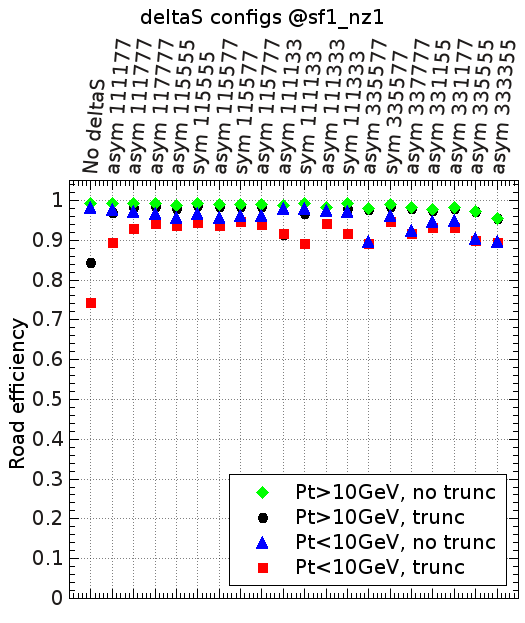
\includegraphics[width=7cm,height=8cm]{AppendixCMSL1TT/figs/final_plots/ttbar_pu200_pt_split_graph}
	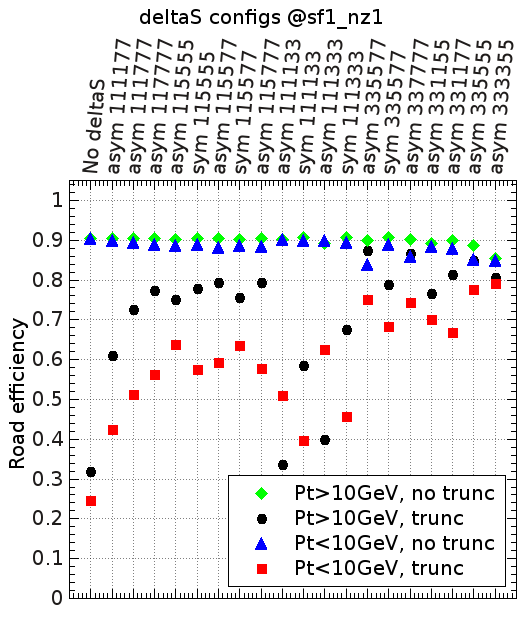
\includegraphics[width=7cm,height=8cm]{AppendixCMSL1TT/figs/final_plots/jet250_pu200_pt_split_graph}
	\label{fig:deltaS_trunc_eff}
\source{The AUTHOR, 2016.}
\end{figure}

In order to make sure that the $sf1\_nz1$ configuration is the best a scan was made for the stub fountain scale factor. It was also included for such scan the ASYM115577 configuration since it looks a better choice for $t\bar{t}+PU200$. The sf scan can be seen in the Fig.~\ref{fig:deltaS_sf_scan}. That plot shows that in fact the ASYM335577 @ $sf1\_nz1$ is an appropriate configuration.

\begin{figure}[htbp]{15cm}
	\caption{Stub fountain scaler factor scan for $t\bar{t}+PU200$.}
	\centering
	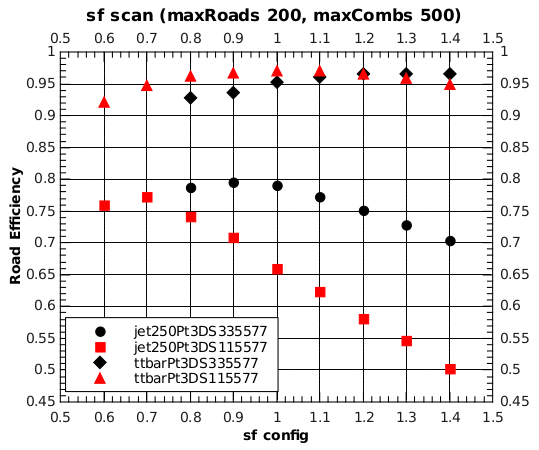
\includegraphics[width=9cm,height=8cm]{AppendixCMSL1TT/figs/sf_scans_with_DS_maxRoads200_maxCombs500}
	\label{fig:deltaS_sf_scan}	
\source{The AUTHOR, 2016.}
\end{figure}


\subsubsection{$\Delta S$ Approach on $\mu$ + PU's}
Studies have been developed about the limits of AM+FPGA approach. It was showed that AM start to lose significant efficiency when PU300/400 is present \footnote{https://indico.cern.ch/event/653731} (even with Hough transform - worst without it). It was worth then to see what $\Delta S$ could do about it. Using the same samples ($\mu$ +PU140, 200, 300, 400) a similar plot was produced to see how the analytical road efficiency is affected by pile up presence when $\Delta S$ is used. The result can be seen in Fig.\ref{fig:deltaS_on_pile_up} where two original plots, without $\Delta S$ approach, were quoted beside the results with stub bending approach. As one can see, with $sf0.8\_nz1$ and 64k or even $sf0.5\_nz1$ with 256k patterns the efficiency loss is high at PU400. Using $\Delta S$ approach the efficiency is $\sim40$ and $\sim20\%$ higher than for sf0.8-64k and sf0.5-256k, respectively. Still an effect persists: low $p_{T}$ is more affected with PU increasing.

\begin{figure}[htbp]{15cm}
	\caption{Muon road efficiency versus pile up. The two first plots (left side) are the results without $\Delta S$ approach and the last plot with it (right side).}
	\centering
	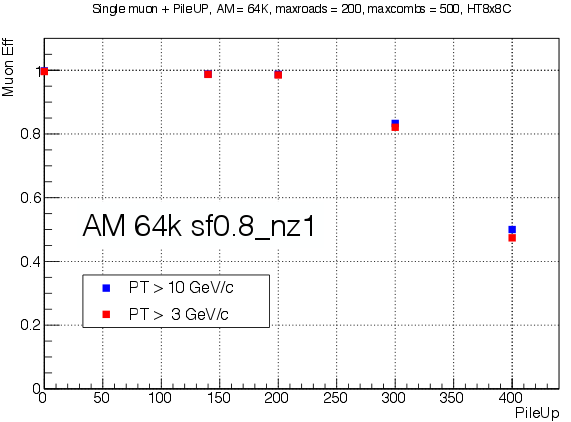
\includegraphics[width=7.5cm,height=7.5cm]{AppendixCMSL1TT/luciano_mupu_sf0p8_plot}\\
	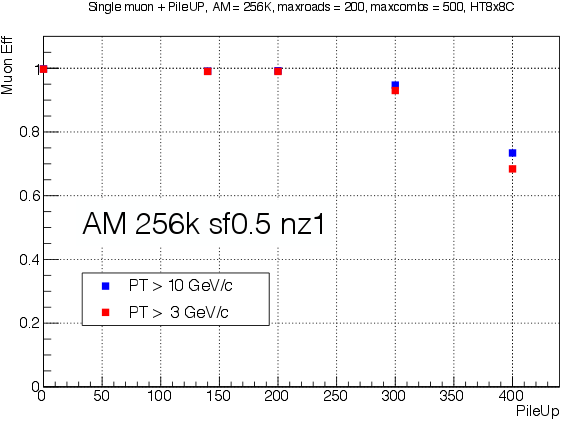
\includegraphics[width=7.5cm,height=7.5cm]{AppendixCMSL1TT/luciano_mupu_sf0p5_plot}\\
	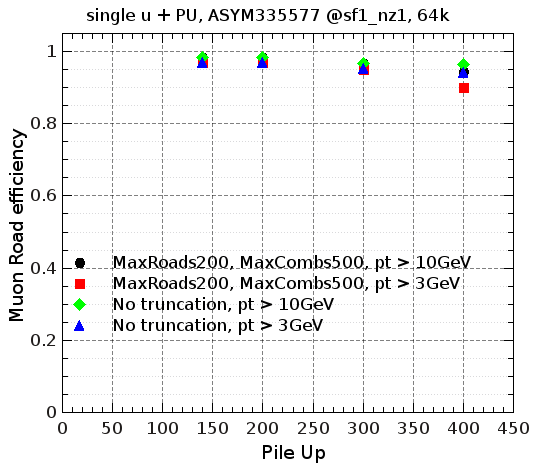
\includegraphics[width=8cm,height=8cm]{AppendixCMSL1TT/figs/muon_road_eff_vs_pile_up_deltaS}
	\label{fig:deltaS_on_pile_up}
\source{The AUTHOR, 2016.}
\end{figure}


\subsubsection{Track Fitter $\chi^{2}$ Revision}
Before proceeding to get final results using $\Delta S$ approach, some stages in the AM package were revisited. The first of them was the track fitter. Currently the tracks $\chi^{2}$ have only a single cut equal to 14.6. However, there are two strong features in the TF $\chi^{2}$: it has two set of constants and its value has a strong dependence on track $p_{T}$ (Fig.~\ref{fig:ttbar_tfchi2_pt}). Then it was decided to redefine the TF $\chi^{2}$ cut. First, the cut should be defined separately for each logic (6/6, 5/6), keeping the cut for 6/6 tight. Also, the cut should be parameterized in terms of track $p_{T}$ for 5/6. For that 8 $p_{T}$ ranges were chosen: [3, 5], [5, 10], [10, 13], [13, 15], [15, 20], [20, 25], [25, 30], [30, $\infty$]GeV.  Then for 6/6 it was decided to take the 99$\%$ of the theoretical $\chi^{2}_{ndof=8}$ curve (Eq.~\ref{eq:chi2_eq}) being equal to 20.2. Fig.~\ref{fig:6b6_chi2_pt} shows how the all 6/6 reconstructed muon tracks (from $t\bar{t}+PU200$) behave compared to the expected distribution. Note that here no DR was used.

\begin{figure}[htbp]{15cm}
	\caption{Track fitter $\chi^{2}$ from all muon tracks in $t\bar{t}+PU200$ versus track $p_{T}$.}
	\centering
	\begin{overpic}
		[scale=0.4]{AppendixCMSL1TT/figs/tfChi2_Pt_all}
		\put(60,70){\color{blue}$t\bar{t}+PU200$}
	\end{overpic}
	\label{fig:ttbar_tfchi2_pt}
\source{The AUTHOR, 2016.}
\end{figure}

\begin{landscape}
\begin{figure}[htbp]{24cm}
	\caption{TF $\chi^{2}$ distribution for 6/6 muon tracks in each track $p_{T}$ range from $t\bar{t}+PU200$.}
	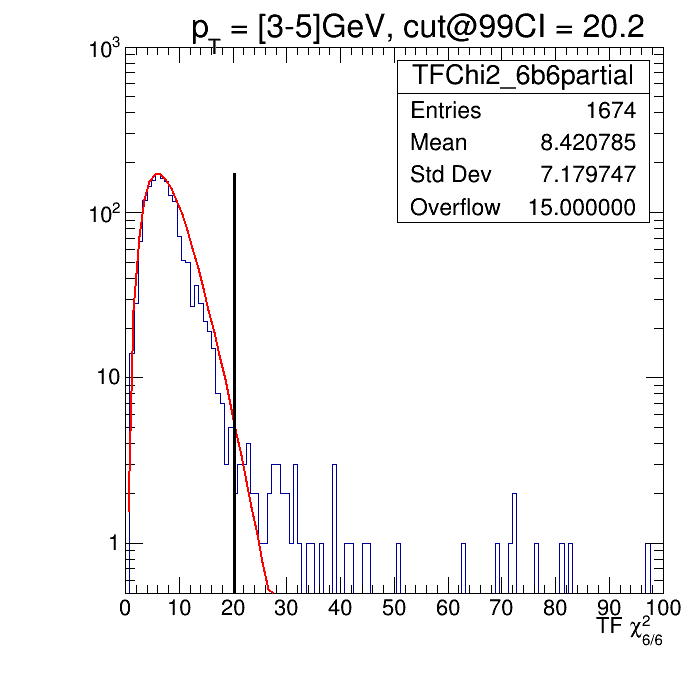
\includegraphics[scale=0.25,trim={1cm 0cm 1cm 0cm},clip]{AppendixCMSL1TT/figs/chi2_6b6_3to5_99cut}
	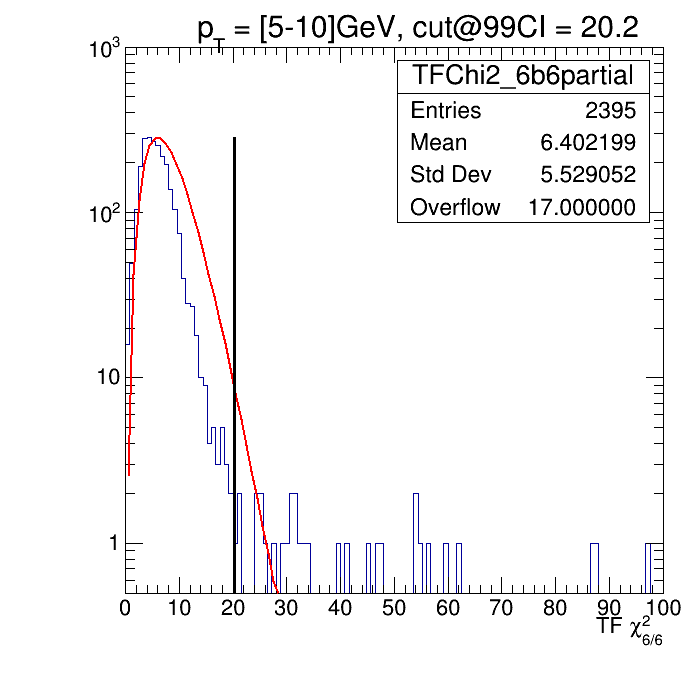
\includegraphics[scale=0.25,trim={1cm 0cm 1cm 0cm},clip]{AppendixCMSL1TT/figs/chi2_6b6_5to10_99cut}	
	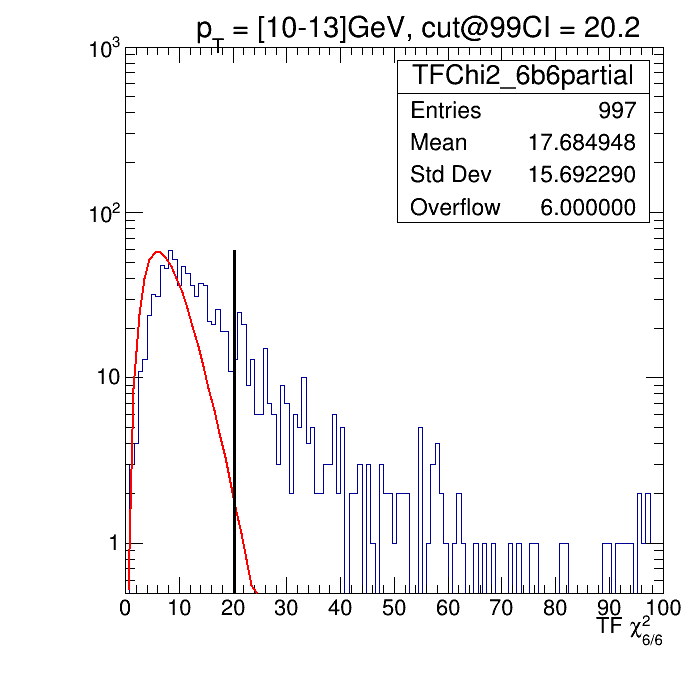
\includegraphics[scale=0.25,trim={1cm 0cm 1cm 0cm},clip]{AppendixCMSL1TT/figs/chi2_6b6_10to13_99cut}		
	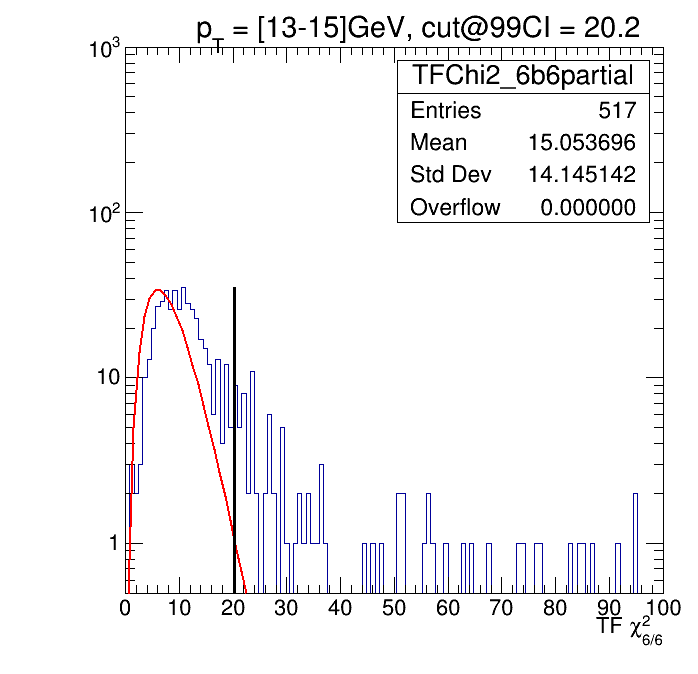
\includegraphics[scale=0.25,trim={1cm 0cm 1cm 0cm},clip]{AppendixCMSL1TT/figs/chi2_6b6_13to15_99cut}\\	
	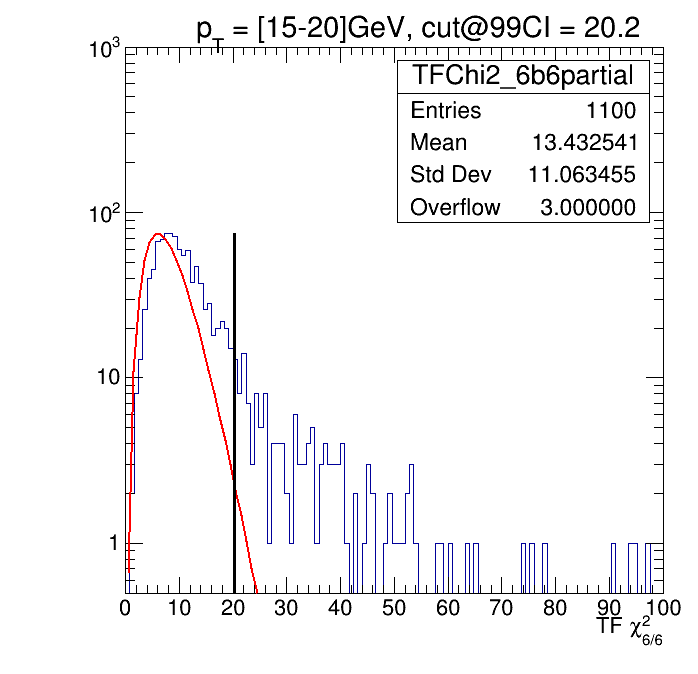
\includegraphics[scale=0.25,trim={1cm 0cm 1cm 0cm},clip]{AppendixCMSL1TT/figs/chi2_6b6_15to20_99cut}	
	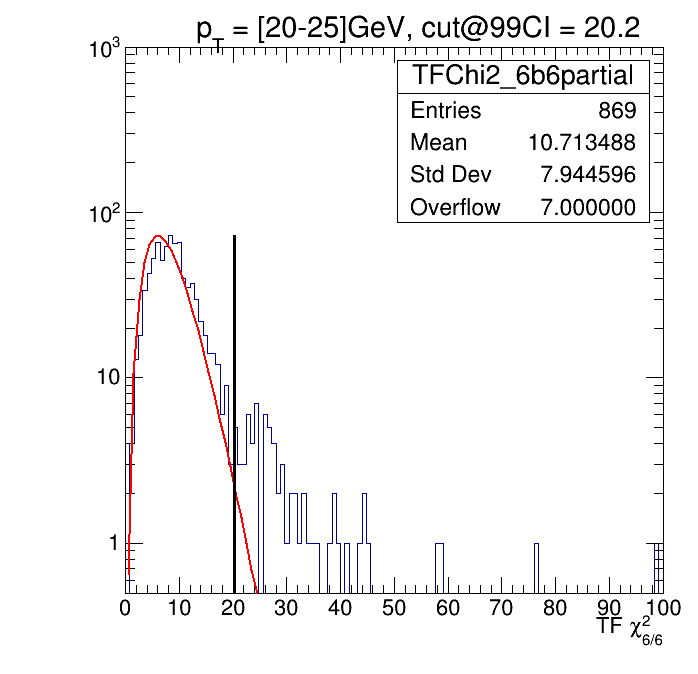
\includegraphics[scale=0.25,trim={1cm 0cm 1cm 0cm},clip]{AppendixCMSL1TT/figs/chi2_6b6_20to25_99cut}	
	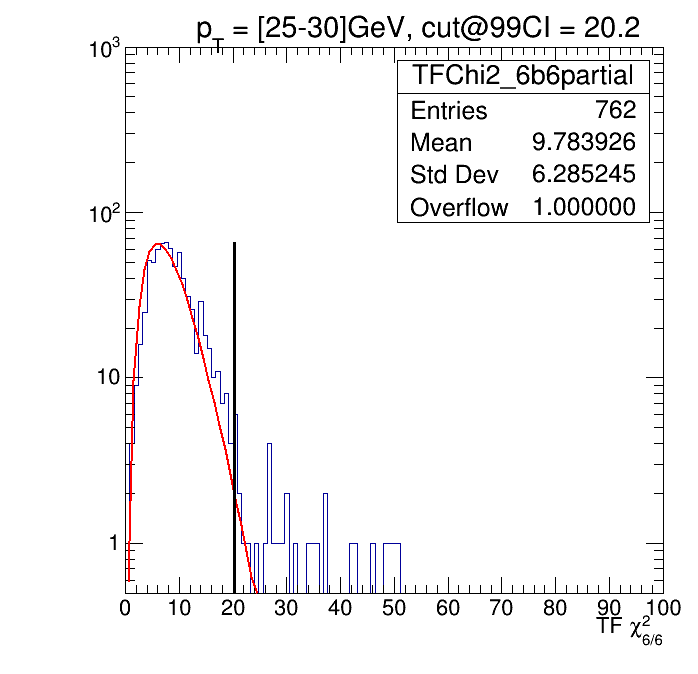
\includegraphics[scale=0.25,trim={1cm 0cm 1cm 0cm},clip]{AppendixCMSL1TT/figs/chi2_6b6_25to30_99cut}	
	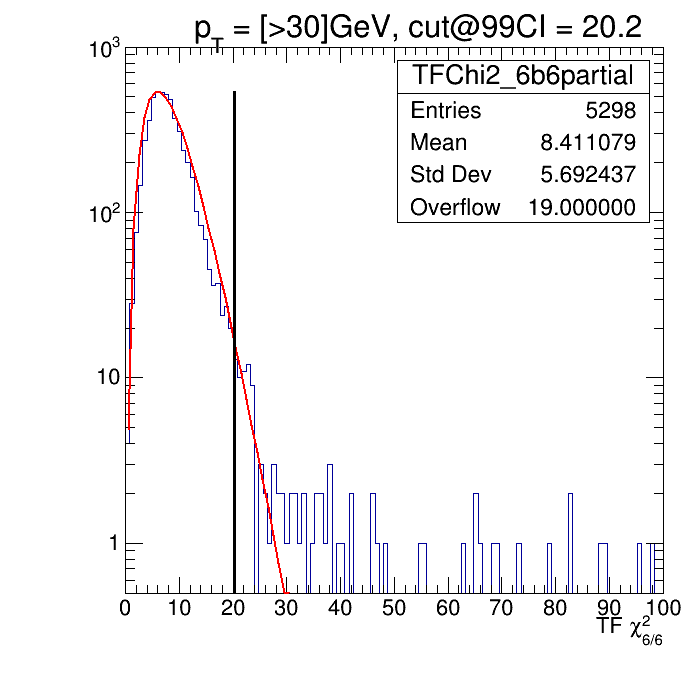
\includegraphics[scale=0.25,trim={1cm 0cm 1cm 0cm},clip]{AppendixCMSL1TT/figs/chi2_6b6_30toInf_99cut}
	\label{fig:6b6_chi2_pt}	
\source{The AUTHOR, 2016.}
\end{figure}
\end{landscape}

\begin{equation}
\label{eq:chi2_eq}
\chi^{2} = \frac{x^{k/2 - 1}}{2^{k/2}~.\Gamma(k/2)~.e^{x/2}},\quad k = degrees~of~freedom
\end{equation}

The normalization of the expected distribution was made by applying a scale factor to the Eq.~\ref{eq:chi2_eq} such that its maximum was equal to the maximum observed (the maximum in each histogram). As it can be seen in the plots, the distributions from some $p_{T}$ ranges are wider or tinner than the expected curve. Such behavior matches with Fig.~\ref{fig:ttbar_tfchi2_pt}. The TF $\chi^{2}$ has higher values for low $p_{T}$ tracks (<5GeV) and in the transition region (>10GeV). Also, the tail in the 6/6 $\chi^{2}$ distribution in disagreement with the expected curve shows that many bad stubs are being accepted with a cut of 14.6. 
The cut for 5/6 tracks were defined finding where the cut should be in order to get $\epsilon_{tracks} = 0.99*\epsilon{roads}$ for each $p_{T}$ range. The distributions for $t\bar{t}+PU200$ and the cuts found for it are in Fig.~\ref{fig:5b6_chi2_pt}. Those cuts were implemented in the package and used to fit tracks in the further studies.

\begin{landscape}
\begin{figure}[htbp]{24cm}
	\caption{TF $\chi^{2}$ distribution for 5/6 muon tracks in each track $p_{T}$ range from $t\bar{t}+PU200$. Vertical bars point the cuts defined.}
	\centering
	\begin{overpic}	
		[scale=0.7]{AppendixCMSL1TT/figs/ttbar_5b6_TFchi2_cuts}
		\put(7,40){\scriptsize$\chi^{2}_{TF,5/6}$ = 15.8}
		\put(33,40){\scriptsize$\chi^{2}_{TF,5/6}$ = 8.5}
		\put(57,40){\scriptsize$\chi^{2}_{TF,5/6}$ = 54.9}
		\put(83,40){\scriptsize$\chi^{2}_{TF,5/6}$ = 36.1}
		\put(7,14){\scriptsize$\chi^{2}_{TF,5/6}$ = 24.7}
		\put(33,14){\scriptsize$\chi^{2}_{TF,5/6}$ = 18.6}
		\put(57,14){\scriptsize$\chi^{2}_{TF,5/6}$ = 14.4}
		\put(83,14){\scriptsize$\chi^{2}_{TF,5/6}$ = 11.4}
	\end{overpic}
	\label{fig:5b6_chi2_pt}
\source{The AUTHOR, 2016.}
\end{figure}
\end{landscape}


\subsubsection{Synthetic Efficiency}
Currently in the AM simulation package there are two methods to compute track reconstruction efficiency: analytic and synthetic. The analytic approach is based only on stubs produced by the tracking particles. It's threshold is 5 stubs, that is, a tracking particle (MC truth track) only can be matched to reconstructed tracks (AM track) that have at least 5 stubs belonging to the tracking particle. The synthetic efficiency approach uses only the four track parameters ($q/p_{T}$, $\phi_0$, $z_{0}$ and $cot~\theta$) to determine the AM track compatibility with a MC track. That is an important way to measure the efficiency because it happens that a stub belonging to a different MC tracking particle can build up a good combination with the other stubs, producing then a track that has compatible parameters (within track resolutions) to the desired MC tracking particle. In the AM package the synthetic efficiency is encoded in the module \textbf{MCTruthAssociator.cc} and it's called during tracking fit stage after the fit. 

The base of synthetic efficiency is described by an algorithm that defines how to pair the collections of MC and AM tracks. Its current structure implemented in the AM package is the following:

\begin{itemize}
	\item [1-] Sort AM tracks with 6/6 first and 5/6 last, and in each group sort by decreasing $p_{T}$;
	\item [2-] Sort MC tracks by decreasing $p_{T}$;
	\item [3-] For each MC track, scan the collection of AM tracks to find those ones that satisfy certain cuts on all four track parameters:
	\begin{itemize}
		\item Flag the AM track that gives the best match as \textbf{good};
		\item Flag all remaining AM tracks matching to a same MC track as \textbf{duplicate};
	\end{itemize}
	\item [4-] Once all MC tracks have been scanned, flag as \textbf{fake} all remaining AM track that is not marked as \textbf{good} or \textbf{duplicate}.
\end{itemize}

From such algorithm the definition of synthetic efficiency is eminent. The denominator is the number of MC tracks. The numerator is the number of AM tracks marked as \textbf{good}. In order to measure the track compatibility and decide which one gives the best match a metric is need. Such metric was created via a $\chi^2$-like formula. Then each AM track paired to a MC track receives a rank that is computed based on the differences in the four track parameters ($\delta p_{i}$) normalized by their respective resolutions. The resolutions were determined by parameterizing the $\delta p_{i}$ in function of $q/p_{T}$. For such task only single particle (no PU) events and only 6/6 tracks were used since they are expected to reproduce the original track parameters with better precision. The $\delta p_{i}$'s in each track parameter were fitted with the same function (constant+gaussian) for different $p_{T}$ ranges, producing the points showed in Fig.~\ref{fig:resolutions}. The dependence on $q/p_{T}$ is stronger for $q/p_{T}$ and $\phi$ parameters. For $z_{0}$ and $cot~\theta$ it is small but the points can still be described with the same function. As one can see the function parameters are not too different between different event types and its shape is approximately the same, even when PU is added. Since pion tracks are the majority of tracks reaching the detector in particle collisions and a common function for all event types is appropriate to be defined, the function parameters from pions (Tab.~\ref{tab:resolution_function_parameters}) were taken.  After that a pseudo-$\chi^{2}$ (usually called $\chi^{2}_{match}$) was defined allowing one to control the tracking matching window.

\begin{figure}[htbp]{16cm}
\caption{Track parameters resolution as function of $q/p_{T}$ for single pion no PU (first column), single muon no PU (second column) and single electron no PU (last column). From top to bottom the track parameters are $q/p_{T}$, $\phi_{0}$, $z_{0}$ and $cot~\theta$.}
\centering
\begin{overpic}
[scale=0.28]{AppendixCMSL1TT/figs/r_qbpT_fit_single_pion_nopu}
\put(50,90){\color{blue}pions}
\end{overpic}
\begin{overpic}
[scale=0.28]{AppendixCMSL1TT/figs/r_qbpT_fit_single_muon_nopu}
\put(50,90){\color{blue}muons}
\end{overpic}
\begin{overpic}
[scale=0.28]{AppendixCMSL1TT/figs/r_qbpT_fit_single_electron_nopu}
\put(45,90){\color{blue}electrons}
\end{overpic}\\
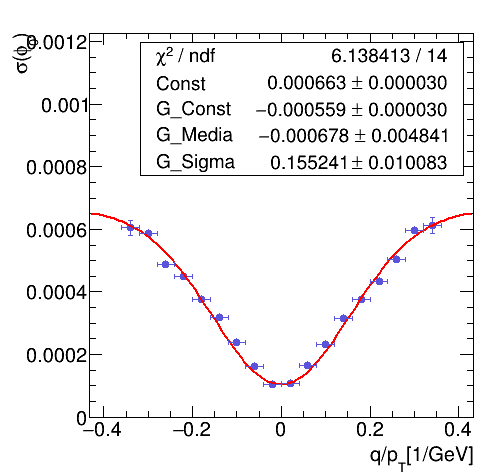
\includegraphics[scale=0.28]{AppendixCMSL1TT/figs/r_phi0_fit_single_pion_nopu}
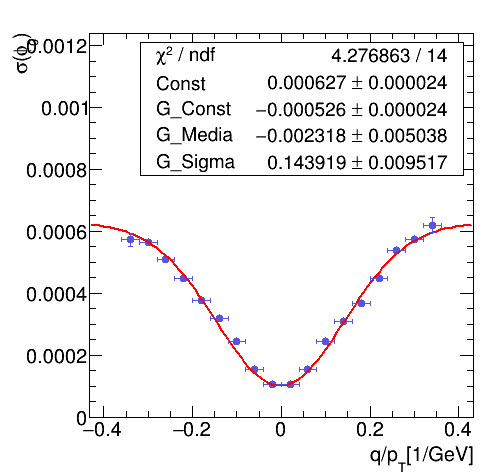
\includegraphics[scale=0.28]{AppendixCMSL1TT/figs/r_phi0_fit_single_muon_nopu}
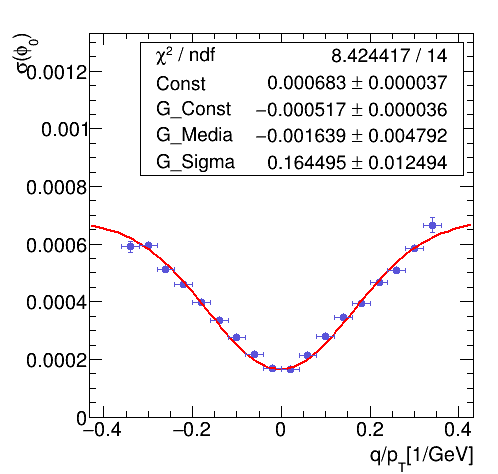
\includegraphics[scale=0.28]{AppendixCMSL1TT/figs/r_phi0_fit_single_electron_nopu}\\
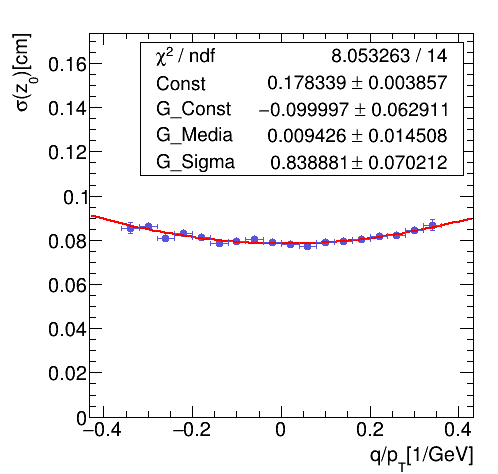
\includegraphics[scale=0.28]{AppendixCMSL1TT/figs/r_z0_fit_single_pion_nopu}
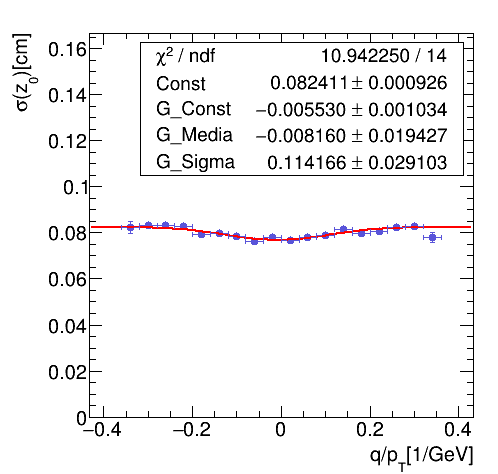
\includegraphics[scale=0.28]{AppendixCMSL1TT/figs/r_z0_fit_single_muon_nopu}
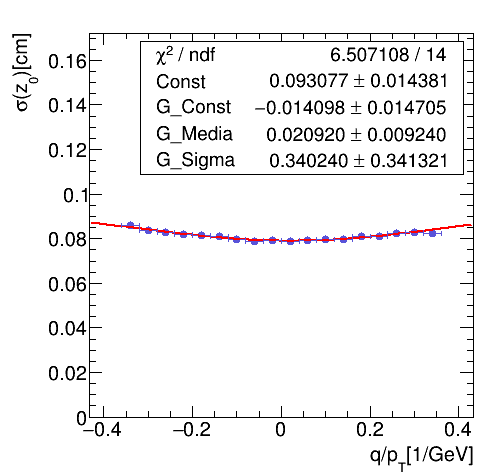
\includegraphics[scale=0.28]{AppendixCMSL1TT/figs/r_z0_fit_single_electron_nopu}\\
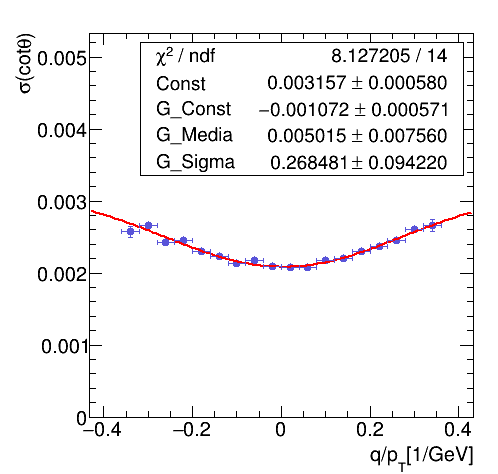
\includegraphics[scale=0.28]{AppendixCMSL1TT/figs/r_cotTheta_fit_single_pion_nopu}
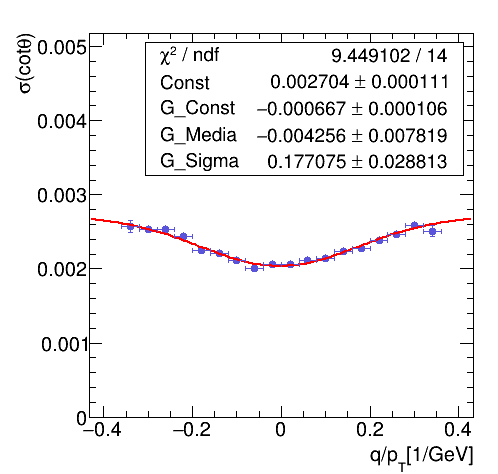
\includegraphics[scale=0.28]{AppendixCMSL1TT/figs/r_cotTheta_fit_single_muon_nopu}
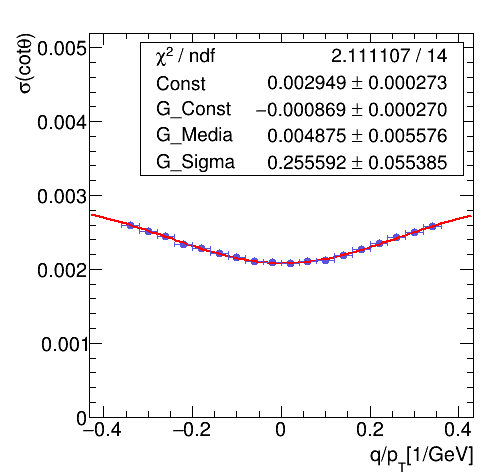
\includegraphics[scale=0.28]{AppendixCMSL1TT/figs/r_cotTheta_fit_single_electron_nopu}
\label{fig:resolutions}	
\source{The AUTHOR, 2016.}
\end{figure}

\begin{table}[htbp]{15cm}
	\caption{Track resolution function parameters from single pion no PU.}
	\centering
	Resolution function: $\Omega(q/p_{T}) = c1 + c2*Gaus(q/p_{T}, \mu, \sigma)$\\
	\begin{tabular}{c|c|c|c|c}
		\hline
		Parameter & $q/p_{T}$ & $\phi_{0}$ & $z_{0}$   & $cot~\theta$\\ 
		\hline
		\hline
		$c_{1}$   & 0.001702  & 0.000663   & 0.178339  & 0.003157\\
		$c_{2}$   & -0.001517 & -0.000559  & -0.099997 & -0.001072\\
		$\mu$     & 0.000256  & -0.000678  & 0.009426  & 0.005015\\
		$\sigma$  & 0.148572  & 0.155241   & 0.838881  & 0.268481\\
		\hline
	\end{tabular}
	\label{tab:resolution_function_parameters}
\source{The AUTHOR, 2016.}

\end{table}

The $\chi^{2}_{match}$ correlates the four track parameters through the following formula,
\begin{equation}
	\chi^{2}_{match} = \sum_{i=0}^{4} \frac{\delta^{2}p_{i}}{\Omega^{2}(q/p_{T})_{i}}, 
	\quad
	\delta p_{i} = (p_{i}^{MC}-p_{i}^{Reco})
\end{equation}
where $p^{MC}_{i}$ ($p^{Reco}_{i}$) stands for the four track parameters from MC (Reco) tracks. Just for completeness the $\chi^{2}_{match}$ is divided by the number of track parameters, that is, four. This reduced $\chi^{2}_{match}$ then gives a ruler for the synthetic efficiency. Once a cut is chosen it defines where the good, duplicate and fake tracks sit. Tracks under such threshold will be good or duplicate and tracks above it will be fake tracks.

First time the cut was chosen based on the capability of finding $99\%$ of the pion tracks, being at $\chi^{2}_{match}/ndof$ = 12.8. As one can see in Fig.~\ref{fig:match_chi2_pion_muon_distribution} it's a good cut even when PU140 is present. Also, it's good for muon case as expected since it's not a busier environment. Using such cut, a group of 4 different event types (muon, pion, electron and pure PU) with different PU levels could be characterized in terms of tracks category (good/duplicate/fake) and track reconstruction efficiency. In Fig.~\ref{fig:track_cat_eff_muon_no_pu} one can see an example. The turn-on at low $p_{T}$ range (3 to ~6GeV) in the efficiencies is associated to another effect and not due to tightness of the synthetic match cut. It has to do with trigger tower definition and will not be discussed here.

\begin{figure}[htbp]{15cm}
	\caption{$\chi^{2}_{match}$ distribution from single pion and single muon event without and with PU.}
	\centering
	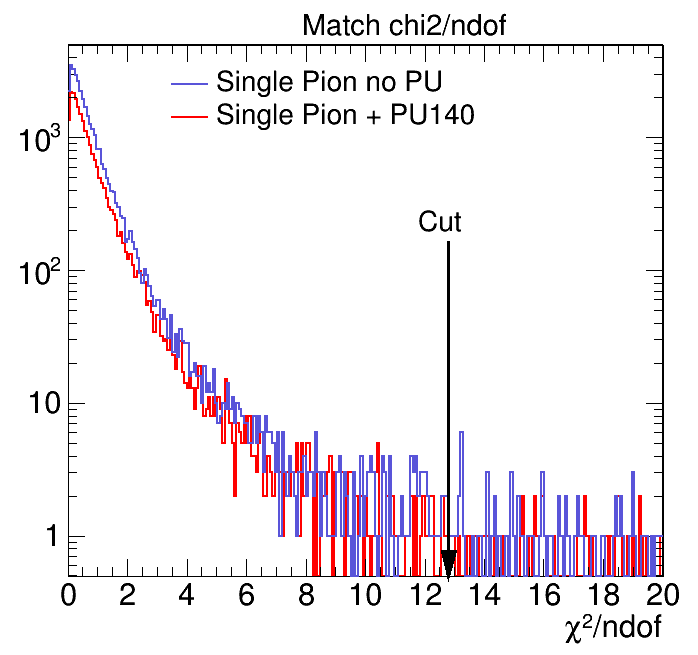
\includegraphics[scale=0.23]{AppendixCMSL1TT/figs/chi2_ndof_single_pion_nopu_pu140}
	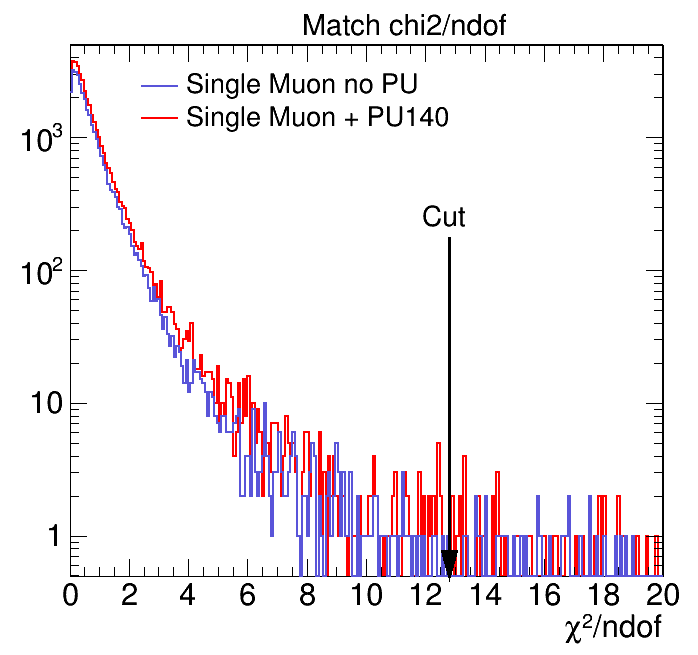
\includegraphics[scale=0.23]{AppendixCMSL1TT/figs/chi2_ndof_single_muon_nopu_pu140}
	\label{fig:match_chi2_pion_muon_distribution}
\source{The AUTHOR, 2016.}
\end{figure}

\begin{figure}[htbp]{15cm}
	\caption{AM track characterization and synthetic efficiency from single muon no PU events.}	
	\centering
	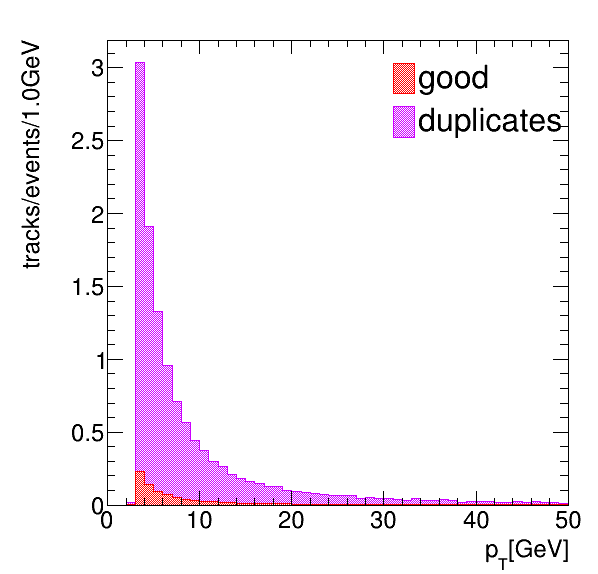
\includegraphics[scale=0.23]{AppendixCMSL1TT/figs/single_muon_nopu_tcat/am_tracks_categorization_vs_pt_allogics_nodupremoval}
	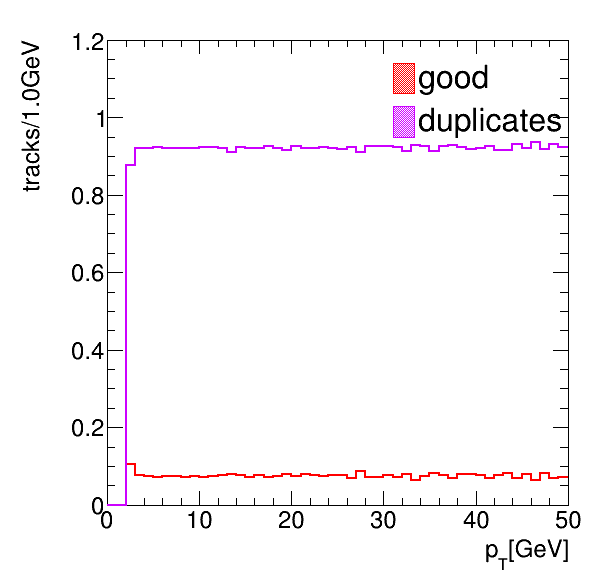
\includegraphics[scale=0.23]{AppendixCMSL1TT/figs/single_muon_nopu_tcat/am_tracks_ratio_vs_pt_allogics_nodupremoval}
	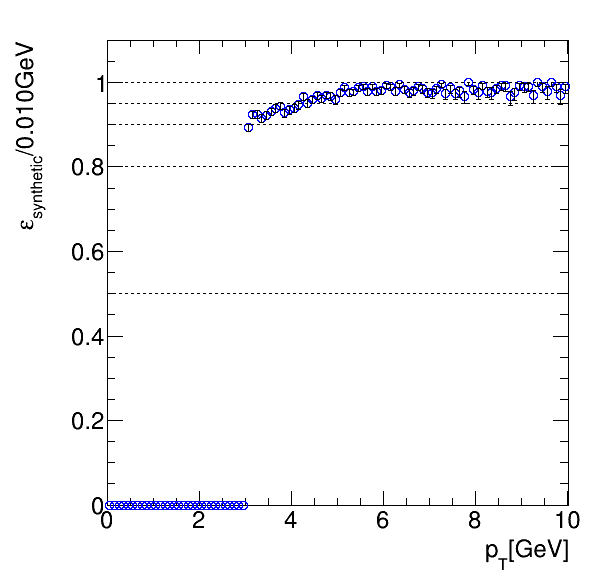
\includegraphics[scale=0.23]{AppendixCMSL1TT/figs/single_muon_nopu_tcat/am_tracks_reco_eff_vs_pt_allogics_nodupremoval}
	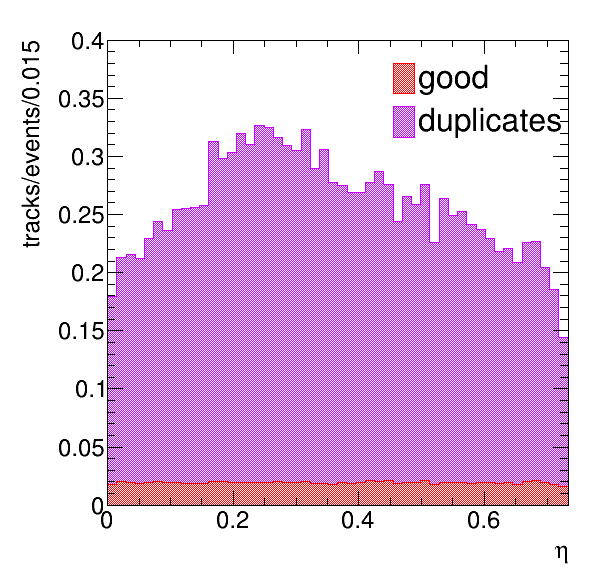
\includegraphics[scale=0.23]{AppendixCMSL1TT/figs/single_muon_nopu_tcat/am_tracks_categorization_vs_eta_allogics_nodupremoval}
	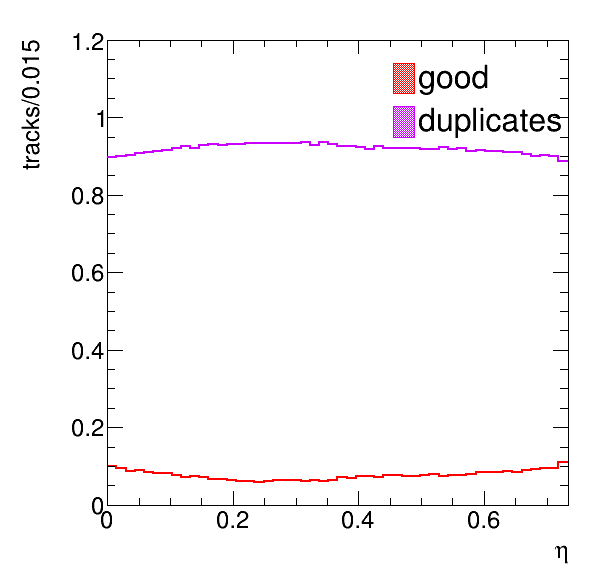
\includegraphics[scale=0.23]{AppendixCMSL1TT/figs/single_muon_nopu_tcat/am_tracks_ratio_vs_eta_allogics_nodupremoval}
	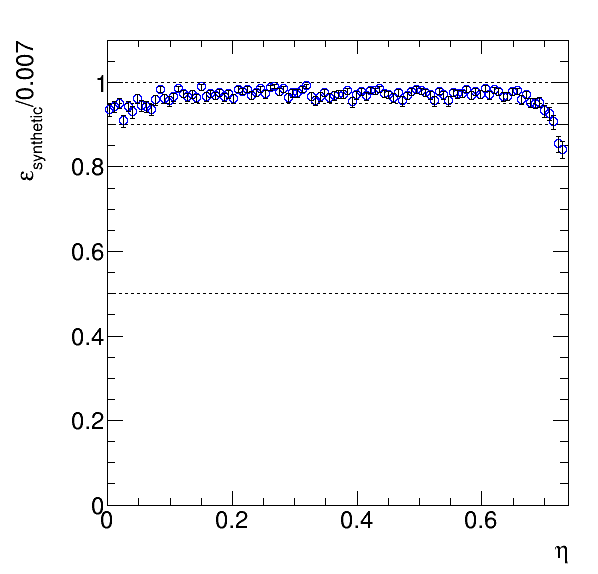
\includegraphics[scale=0.23]{AppendixCMSL1TT/figs/single_muon_nopu_tcat/am_tracks_reco_eff_vs_eta_allogics_nodupremoval}
	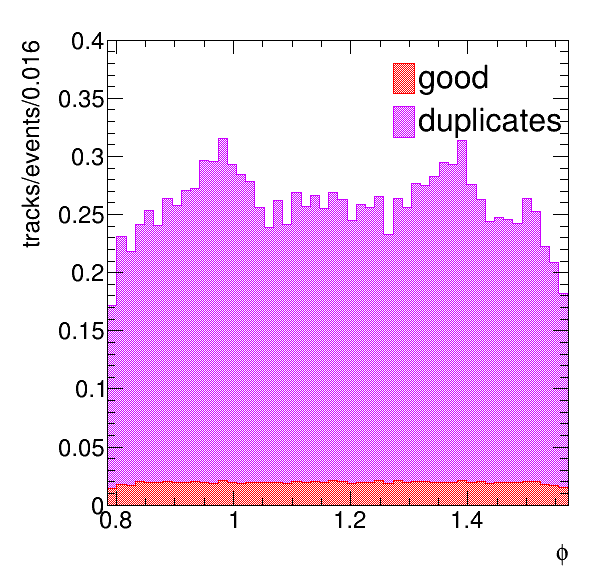
\includegraphics[scale=0.23]{AppendixCMSL1TT/figs/single_muon_nopu_tcat/am_tracks_categorization_vs_phi_allogics_nodupremoval}
	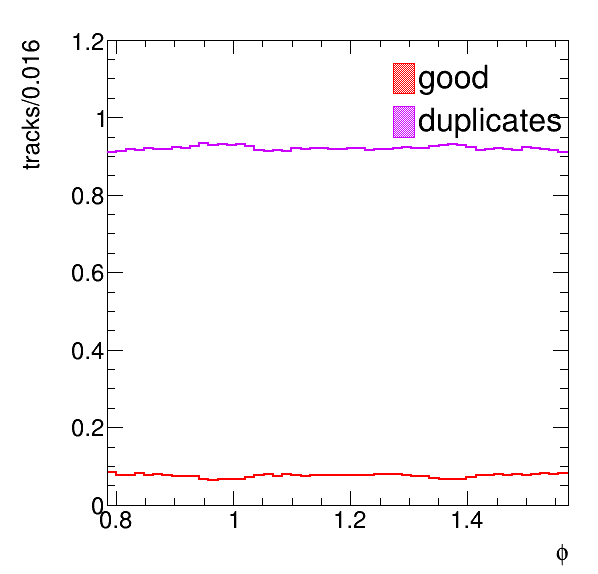
\includegraphics[scale=0.23]{AppendixCMSL1TT/figs/single_muon_nopu_tcat/am_tracks_ratio_vs_phi_allogics_nodupremoval}
	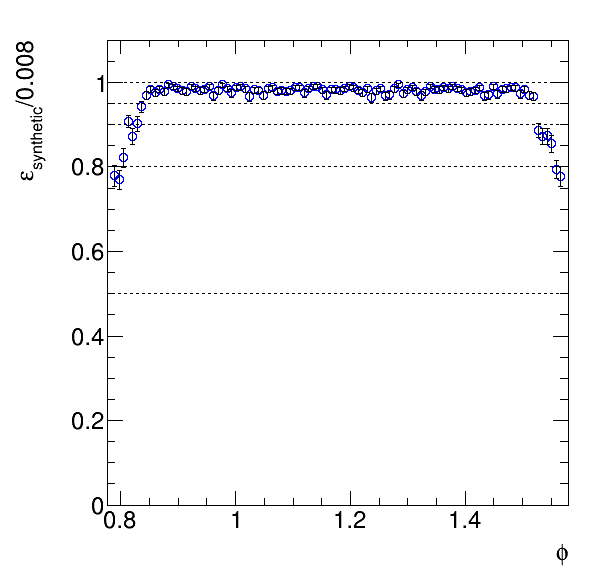
\includegraphics[scale=0.23]{AppendixCMSL1TT/figs/single_muon_nopu_tcat/am_tracks_reco_eff_vs_phi_allogics_nodupremoval}
	\label{fig:track_cat_eff_muon_no_pu}
\source{The AUTHOR, 2016.}
\end{figure}

In the track files created by AM package there are three branches that store important information from synthetic approach. Currently, the branch \textbf{AMTTTracks\_synMatchCat} stores an integer that tags AM track category: 1 for good tracks, -1 for duplicates and -2 for fakes. The branch \textbf{AMTTTracks\_synTpId} stores the tracking particle index in a event to which the AM track was matched (good or duplicate). Index equal to -1 means that the AM track is fake, that is, it could not match to any MC tracking particle then it can't have an index. The branch \textbf{AMTTTracks\_matchChi2} stores the $\chi^{2}_{match}$ value for AM tracks flagged as a good or duplicate track. For fake tracks the value is 999999999.

\subsubsection{$\chi^{2}_{match}$ Optimization and Synthetic-Analytical Methods Connection}
In order to better decide the cut to be used on the $\chi^{2}_{match}$, avoiding then random combinations of stubs but without loosing efficiency in busier event a new strategy was designed. It also allowed an unification between analytical and synthetic approaches. Such strategy consisted on scanning through different cuts on $\chi^{2}_{match}$ and observing how the synthetic efficiency and the fraction of good/duplicate/fake tracks change. It's intuitive that a very restrictive cut will cause loss of efficiency making good tracks being classified as fake. On the other direction a very loose cut will make tracks with quite different parameters to be matched, so real fake tracks will be classified as good or duplicate and duplicate tracks can be classified as good ones. 

Other quantity that was monitored through those scannings was the fraction of truth stubs in the AM tracks being classified as good or duplicate. That fraction was computed checking how many stubs the AM track had in common with the matching MC track. Both of those informations can be seen in Fig.~\ref{fig:chi2_match_optimization}. The notation used in those plots are track category and number of stubs. For instance, \textbf{GOOD 6S} stands for AM tracks flagged as good and have 6 stubs that come from the matching tracking particle (the same for the duplicates). The plots on the top show that a very restrictive cut on $\chi^{2}_{match}$ produces many fake tracks as it's too tight to compensate the track parameters resolution. Once the cut starts to increase the fraction of fake tracks quickly gets reduced while it's possible to see the fraction of duplicates and the synthetic efficiency increasing (as the fraction of good tracks also slowly increases). After that the three curves reduces their slope - the synthetic efficiency becomes actually flat. Then, on $\chi^{2}_{match} \sim$ 1k the curves start to change faster again and after 10k the fraction of good tracks increases abruptly and duplicates decrease abruptly. A last thing to notice is the flat region for synthetic efficiency in the plots for $\mu$ +PU200 and +PU400. It looks quite similar, showing no strong dependence on PU.

Looking into the bottom plots one see what happens in the previous stages through the analytical view. First thing to make clear is that, in that plot the number of stubs stated in the legends means the number of stubs belonging to the tracking particle that the AM track was matched - and not the actual number of stubs the track has. Then, the second thing to notice is that the majority of AM tracks have 5 stubs coming from the tracking particle (either good or duplicate tracks) - if the AM track is a 6/6, it means that the track has one stub from other tracking particle. In such case, that majority comes from three sources: one is that naturally there are more 5/6 than 6/6 tracks, two is that the advanced combination builder produces 5/6 combinations from all 6/6 combinations and three is that a 6/6 AM track may not have 6 stubs from the same tracking particle. In the frame of synthetic efficiency the most significant result is the fraction of tracks that don't have any stub coming from the tracking particle to which it was matched (GOOD 0S and DUPLICATE 0S). In other words, the $\chi^{2}_{match}$ cut is too loose that random combinations of stubs are being flagged as a track. So, for sure one needs to avoid that region which imposes an upper limit on $\chi^{2}_{match}$ = 100 based on the plot for jets. For $\mu$ is not so evident maybe because of the muon track is more un-like a pion track (that essentially composes the pile up). While, for jets, is more susceptible to occur that a pion track ends up reconstructed with stubs coming from other pion. Currently, an flag was developed to control the $\chi^{2}_{match}$ cut. Its default value is 40 that was agreed to be the adequate cut based on Fig~\ref{fig:chi2_match_optimization}. An user can change it during simulation actioning the flag \textbf{$--$maxChi2Match} followed by the cut value.

\begin{figure}[htbp]{16cm}
	\caption{AM tracks categories fraction and truth stub fraction versus $\chi^{2}_{match}$ cut for $\mu+PU200$ on left column and for $jet(p_{T}=250GeV) + PU200$ on right column.}
	\centering
	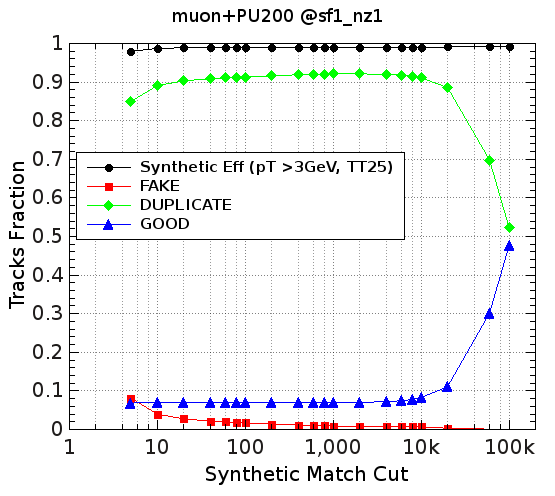
\includegraphics[width=7.5cm,height=6.7cm]{AppendixCMSL1TT/figs/final_plots/mupu200_synthetic_view}
	\includegraphics[width=7.5cm,height=6.7cm]{AppendixCMSL1TT/figs/final_plots/mupu200_analytic_view}\\
	\includegraphics[width=7.5cm,height=6.7cm]{AppendixCMSL1TT/figs/final_plots/mupu400_synthetic_view}
	\includegraphics[width=7.5cm,height=6.7cm]{AppendixCMSL1TT/figs/final_plots/mupu400_analytic_view}\\
	\includegraphics[width=7.5cm,height=6.7cm]{AppendixCMSL1TT/figs/final_plots/jet250pu200_synthetic_view}
	\includegraphics[width=7.5cm,height=6.7cm]{AppendixCMSL1TT/figs/final_plots/jet250pu200_analytic_view}
	\label{fig:chi2_match_optimization}
\source{The AUTHOR, 2016.}
\end{figure}


\subsubsection{Duplicate Removal (DR) Based on Stubs}
The duplicate removal was designed to mitigate tracks replicas. Those are tracks that are very similar between them, sharing equal stubs and usually having equal/similar parameters. In the level of AM work structure, those tracks arise due to stubs combinatorics (from the same road) generated (in tracking fit stage) in order to find out the appropriate group of stubs coming from a real track. A road can also have extra stubs due to secondary radiation from original tracking particle or due to different particles crossing the same detector region that comprehends an expected pattern. As mentioned, the advanced combination builder generates 5/6 combinations from 6/6. Those 5/6 combinations are also duplicates. 

The DR based on stubs is an analytical approach since it uses the stubs shared between different tracks. It's current algorithm is:

\begin{itemize}
	\item [1-] Take the first AM track and store it into a new list (unique tracks list);
	\item [2-] Then compare each remaining AM track to the tracks stored in the unique tracks list:
	\begin{itemize}
		\item If an AM track and an unique track have more equal stubs than allowed remove the AM track;
		\item Else, add the AM track into the unique tracks list;
	\end{itemize}
	\item [3-] Repeat the precess until all AM tracks have been scanned.
\end{itemize}

A scan on the DR option was made monitoring the fraction of AM track categories per event and the synthetic efficiency for three samples: $\mu$, $t\bar{t}$ and jet +PU200. The synthetic efficiency was computed using only the muons from $\mu$ and $t\bar{t}$ +PU200 samples, while for jet sample all tracks are included in the computation. The results are showed in Tab.~\ref{tab:dr_scan_tables}. From them, first important thing to notice is the ratio of synthetic efficiency and the track efficiency. The track efficiency is the analytical efficiency computed using the tracks, that is, a tracking particle is considered found if at least a combination has at least 5 stubs coming from it.  As expected the synthetic efficiency is slightly higher than the analytical efficiency due to extra stubs.

The numbers also show that the majority of the duplicate tracks have 4 stubs in common with the good tracks since DR options 5 and 4 are not effective on duplicate removal. As it can be seen DR $\leq$ 3 significantly affects the analytical track efficiency although synthetic efficiency reduces very few. That suggests a DR option even more restrictive like DR = 0 (the only one actually capable to completely remove all duplicate tracks). So, it was decided to reduce the DR option previously adopted of 2 to 0. It was also noticed that DR is also removing fake tracks. That is a new and important result since those fake tracks mean hardware latency after all. So, DR will also helps to reduce the AM processing latency. A study from where the extra stubs (that makes synthetic efficiency higher that the analytic one) come from was done. Through it, however, it was discovered that the majority of those stubs come from particle not identified by the current software (\textbf{cmssw}). And a very small fraction come from pions (which ones would be called random stubs since are not expected to be correlated to the $\mu$ - as an irradiated $\gamma$, for instance).

\begin{table}[htbp]{15cm}
	\caption{AM track categories per event versus DR configuration for $\mu+PU200$, $t\bar{t}+PU200$ and $jet(p_{T}=250GeV) + PU200$.}
	\centering
	$\mu+PU200$\\
	\begin{tabular}{c|c|c|c|c|c}
		\hline
		\hline
		DR option & Goods & Duplicates & Fakes & Track eff & Synthetic eff\\
		\hline
		None      & 1.976 &	25.785	   & 0.614 & 0.985	   & 0.989\\
		5         & 1.976 &	25.785	   & 0.614 & 0.985	   & 0.989\\
		4         & 1.976 &	8.898	   & 0.275 & 0.98	   & 0.989\\
		3         & 1.973 &	0.604	   & 0.095 & 0.964	   & 0.989\\
		2         & 1.969 &	0.065	   & 0.047 & 0.953	   & 0.989\\
		1         & 1.967 &	0.007	   & 0.039 & 0.951	   & 0.988\\
		0         & 1.966 &	0.000	   & 0.038 & 0.951	   & 0.988\\
		\hline
	\end{tabular}\\[0.5cm]
	$t\bar{t}+PU200$\\
	\begin{tabular}{c|c|c|c|c|c}
		\hline
		\hline
		DR option & Goods & Duplicates & Fakes & Track eff & Synthetic eff\\
		\hline
		None	  & 3.206 &	43.205	   & 3.252 & 0.981	   & 0.983\\
		5	      & 3.206 &	43.205	   & 3.252 & 0.981     & 0.983\\
		4	      & 3.205 &	14.993	   & 1.384 & 0.976     & 0.983\\
		3	      & 3.197 &	1.023	   & 0.400 & 0.957     & 0.98\\
		2	      & 3.183 &	0.111	   & 0.253 & 0.948     & 0.977\\
		1	      & 3.179 &	0.008	   & 0.230 & 0.945     & 0.976\\
		0	      & 3.178 &	0.000	   & 0.226 & 0.945     & 0.976\\
		\hline
	\end{tabular}\\[0.5cm]
	$jet(p_{T}=250GeV)+PU200$\\
	\begin{tabular}{c|c|c|c|c|c}
		\hline
		\hline
		DR option & Goods & Duplicates & Fakes & Track eff & Synthetic eff\\
		\hline
		None	  & 8.506 &	143.735	   & 8.924 & 0.89	   & 0.897\\
		5	      & 8.506 &	143.735	   & 8.924 & 0.89	   & 0.897\\
		4	      & 8.506 &	52.935	   & 4.109 & 0.883	   & 0.897\\
		3	      & 8.481 &	4.746	   & 1.167 & 0.823	   & 0.895\\
		2	      & 8.431 &	0.642	   & 0.597 & 0.754	   & 0.889\\
		1	      & 8.412 &	0.067	   & 0.506 & 0.738	   & 0.887\\
		0	      & 8.406 &	0.003	   & 0.482 & 0.74	   & 0.886\\
		\hline
	\end{tabular}
	\label{tab:dr_scan_tables}	
\source{The AUTHOR, 2016.}
\end{table}

The DR code is wrote in the \textbf{DuplicateRemoval.cc} module and it has the flag \textbf{$--$rmDuplicate} that can be used to set the maximum number of stubs to be shared between unique tracks. The values must be integers from 0 to 6. The default option is 0 and to set off the DR the user must pass the argument -1 to the flag. Since DR is an analytical approach it acts right after tracking fit stage and before the synthetic match stage being actioned.


\subsubsection{Final FOMs}
In the following pages will be show the common FOMs (figure of merits) usually used to characterize the final performance of AM simulation. Such plots (Fig(s).~\ref{fig:fom_ttbar_pu200}, \ref{fig:fom_jets_pu200}, \ref{fig:fom_mu_pu200}, \ref{fig:fom_mu_pu400}, \ref{fig:fom_mu_pu400}) show the synthetic efficiency for the track reconstruction and the track categories ratios in terms of the track $p_{T}$, $\eta$ and $\phi$. The plots also show the comparison between the standard $sf1\_nz1$ configuration and two chosen $\Delta S$ schemes: ASYM335577 and SYM335577. Also, truncation at 200 roads and 500 combinations is applied.

\begin{figure}[htbp]{16cm}
\caption{Track reconstruction efficiency for $t\bar{t}+PU200$ sample. The pattern bank used had 64k patterns and truncation at 200 roads and 500 combinations has been applied. Duplicate removal was applied by requiring DR=0.}
\centering
\begin{overpic}
	[scale=0.3]{AppendixCMSL1TT/figs/final_plots/ttbarPU200/ttbar_pu200_track_eff_pt_trunc}
	\put(25,45){\color{blue}\tiny$\epsilon_{synthetic}(p_{T}>3GeV)$ = 0.80}
	\put(25,40){\color{red}\tiny$\epsilon_{synthetic}(p_{T}>3GeV)$ = 0.94}
	\put(25,35){\color{violet}\tiny$\epsilon_{synthetic}(p_{T}>3GeV)$ = 0.96}
\end{overpic}
\begin{overpic}
	[scale=0.3]{AppendixCMSL1TT/figs/final_plots/ttbarPU200/ttbar_pu200_track_ratio_pt_trunc}
\end{overpic}\\

\begin{overpic}
	[scale=0.3]{AppendixCMSL1TT/figs/final_plots/ttbarPU200/ttbar_pu200_track_eff_eta_trunc}
\end{overpic}
\begin{overpic}
	[scale=0.3]{AppendixCMSL1TT/figs/final_plots/ttbarPU200/ttbar_pu200_track_ratio_eta_trunc}
\end{overpic}\\	

\begin{overpic}
	[scale=0.3]{AppendixCMSL1TT/figs/final_plots/ttbarPU200/ttbar_pu200_track_eff_phi_trunc}
\end{overpic}	
\begin{overpic}
	[scale=0.3]{AppendixCMSL1TT/figs/final_plots/ttbarPU200/ttbar_pu200_track_ratio_phi_trunc}
\end{overpic}
\label{fig:fom_ttbar_pu200}	
\source{The AUTHOR, 2016.}
\end{figure}


\begin{figure}[htbp]{16cm}
\caption{Track reconstruction efficiency for $jets(p_{T}=250GeV)+PU200$ sample. The pattern bank used had 64k patterns and truncation at 200 roads and 500 combinations has been applied. Duplication removal was applied by requiring DR=0.}
\centering
\begin{overpic}
	[scale=0.3]{AppendixCMSL1TT/figs/final_plots/jet250PU200/jet250_pu200_track_eff_pt_trunc}
	\put(25,45){\color{blue}\tiny$\epsilon_{synthetic}(p_{T}>3GeV)$ = 0.27}
	\put(25,40){\color{red}\tiny$\epsilon_{synthetic}(p_{T}>3GeV)$ = 0.78}
	\put(25,35){\color{violet}\tiny$\epsilon_{synthetic}(p_{T}>3GeV)$ = 0.71}
\end{overpic}
\begin{overpic}
	[scale=0.3]{AppendixCMSL1TT/figs/final_plots/jet250PU200/jet250_pu200_track_ratio_pt_trunc}
\end{overpic}

\begin{overpic}
	[scale=0.3]{AppendixCMSL1TT/figs/final_plots/jet250PU200/jet250_pu200_track_eff_eta_trunc}
\end{overpic}
\begin{overpic}
	[scale=0.3]{AppendixCMSL1TT/figs/final_plots/jet250PU200/jet250_pu200_track_ratio_eta_trunc}
\end{overpic}	

\begin{overpic}
	[scale=0.3]{AppendixCMSL1TT/figs/final_plots/jet250PU200/jet250_pu200_track_eff_phi_trunc}
\end{overpic}	
\begin{overpic}
	[scale=0.3]{AppendixCMSL1TT/figs/final_plots/jet250PU200/jet250_pu200_track_ratio_phi_trunc}
\end{overpic}	
\label{fig:fom_jets_pu200}
\source{The AUTHOR, 2016.}
\end{figure}

\begin{figure}[htbp]{16cm}
\caption{Track reconstruction efficiency for $\mu+PU200$ sample. The pattern bank used had 64k patterns and truncation at 200 roads and 500 combinations has been applied. Duplication removal was applied by requiring DR=0.}
\centering
\begin{overpic}
	[scale=0.3]{AppendixCMSL1TT/figs/final_plots/muPU200/mu_pu200_track_eff_pt_trunc}
	\put(25,45){\color{blue}\tiny$\epsilon_{synthetic}(p_{T}>3GeV)$ = 0.88}
	\put(25,40){\color{red}\tiny$\epsilon_{synthetic}(p_{T}>3GeV)$ = 0.97}
	\put(25,35){\color{violet}\tiny$\epsilon_{synthetic}(p_{T}>3GeV)$ = 0.98}
\end{overpic}
\begin{overpic}
	[scale=0.3]{AppendixCMSL1TT/figs/final_plots/muPU200/mu_pu200_track_ratio_pt_trunc}
\end{overpic}

\begin{overpic}
	[scale=0.3]{AppendixCMSL1TT/figs/final_plots/muPU200/mu_pu200_track_eff_eta_trunc}
\end{overpic}
\begin{overpic}
	[scale=0.3]{AppendixCMSL1TT/figs/final_plots/muPU200/mu_pu200_track_ratio_eta_trunc}
\end{overpic}	

\begin{overpic}
	[scale=0.3]{AppendixCMSL1TT/figs/final_plots/muPU200/mu_pu200_track_eff_phi_trunc}
\end{overpic}	
\begin{overpic}
	[scale=0.3]{AppendixCMSL1TT/figs/final_plots/muPU200/mu_pu200_track_ratio_phi_trunc}
\end{overpic}	
\label{fig:fom_mu_pu200}
\source{The AUTHOR, 2016.}
\end{figure}

\begin{figure}[htbp]{16cm}
\caption{Track reconstruction efficiency for $\mu+PU300$ sample. The pattern bank used had 64k patterns and truncation at 200 roads and 500 combinations has been applied. Duplication removal was applied by requiring DR=0.}
\centering
\begin{overpic}
	[scale=0.3]{AppendixCMSL1TT/figs/final_plots/muPU300/mu_pu300_track_eff_pt_trunc}
	\put(25,60){\color{blue}\tiny$\epsilon_{synthetic}(p_{T}>3GeV)$ = 0.36}
	\put(25,55){\color{red}\tiny$\epsilon_{synthetic}(p_{T}>3GeV)$ = 0.95}
	\put(25,50){\color{violet}\tiny$\epsilon_{synthetic}(p_{T}>3GeV)$ = 0.94}
\end{overpic}
\begin{overpic}
	[scale=0.3]{AppendixCMSL1TT/figs/final_plots/muPU300/mu_pu300_track_ratio_pt_trunc}
\end{overpic}

\begin{overpic}
	[scale=0.3]{AppendixCMSL1TT/figs/final_plots/muPU300/mu_pu300_track_eff_eta_trunc}
\end{overpic}
\begin{overpic}
	[scale=0.3]{AppendixCMSL1TT/figs/final_plots/muPU300/mu_pu300_track_ratio_eta_trunc}
\end{overpic}	

\begin{overpic}
	[scale=0.3]{AppendixCMSL1TT/figs/final_plots/muPU300/mu_pu300_track_eff_phi_trunc}
\end{overpic}	
\begin{overpic}
	[scale=0.3]{AppendixCMSL1TT/figs/final_plots/muPU300/mu_pu300_track_ratio_phi_trunc}
\end{overpic}	
\label{fig:fom_mu_pu300}
\source{The AUTHOR, 2016.}
\end{figure}
	

\begin{figure}[htbp]{16cm}
\caption{Track reconstruction efficiency for $\mu+PU400$ sample. The pattern bank used had 64k and truncation at 200 roads and 500 combinations has been applied. Duplication removal was applied by requiring DR=0.}
\centering
\begin{overpic}
	[scale=0.3]{AppendixCMSL1TT/figs/final_plots/muPU400/mu_pu400_track_eff_pt_trunc}
	\put(25,45){\color{blue}\tiny$\epsilon_{synthetic}(p_{T}>3GeV)$ = 0.10}
	\put(25,40){\color{red}\tiny$\epsilon_{synthetic}(p_{T}>3GeV)$ = 0.89}
	\put(25,35){\color{violet}\tiny$\epsilon_{synthetic}(p_{T}>3GeV)$ = 0.75}
\end{overpic}
\begin{overpic}
	[scale=0.3]{AppendixCMSL1TT/figs/final_plots/muPU400/mu_pu400_track_ratio_pt_trunc}
\end{overpic}

\begin{overpic}
	[scale=0.3]{AppendixCMSL1TT/figs/final_plots/muPU400/mu_pu400_track_eff_eta_trunc}
\end{overpic}
\begin{overpic}
	[scale=0.3]{AppendixCMSL1TT/figs/final_plots/muPU400/mu_pu400_track_ratio_eta_trunc}
\end{overpic}	

\begin{overpic}
	[scale=0.3]{AppendixCMSL1TT/figs/final_plots/muPU400/mu_pu400_track_eff_phi_trunc}
\end{overpic}	
\begin{overpic}
	[scale=0.3]{AppendixCMSL1TT/figs/final_plots/muPU400/mu_pu400_track_ratio_phi_trunc}
\end{overpic}	
\label{fig:fom_mu_pu400}
\source{The AUTHOR, 2016.}
\end{figure}
	

\subsubsection{Generated AM Pattern Banks}
During the studies presented here several pattern banks have been generated and for the information of the reader and even possible reference, the properties of such banks are summarized in this section through the Tab(s).~\ref{tab:banks_info_noDS}, \ref{tab:banks_info_DS} and the Fig.~\ref{fig:pattern_banks_comparison}. As presented along the text it was decided to work around the configuration $sf1\_nz1$, which has a good road efficiency (as shown in Fig.~\ref{fig:deltaS_sf_scan}) to develop the stub bending approach and that is why, in the tables, the notation for the stub bending approach only appears for that particular configuration. Fig.~\ref{fig:pattern_banks_comparison} compares the size of the banks for the standard $sf1\_nz1$ and its variants with the application of the stub bending approach. As it is expected such approach increases the number of pattern due to the extra parameter assigned to each stub (remember, that, though, does not increase the partition of the detector).

\begin{table}[htbp]{15cm}
	\caption{AM pattern banks size for different configurations and coverages. The configurations stands for the way the CMS detector is partitioned in \textit{$\phi$} and \textbf{z} directions. The coverage stand for the fraction of track reconstructed over the total number of track patterns in a given configuration.}
	\centering
	\begin{tabular}{c|c|c|c}
		\hline
		\hline
		Bank         & @90     & @95     & @99\\
		\hline
		$sf0.3\_nz1$ & 1011898 & 1408735 & 2393133\\
		$sf0.4\_nz1$ & 385610  & 527271  & 857645\\		
		$sf0.5\_nz1$ & 197421  & 265719  & 419641\\
		$sf0.6\_nz1$ & 119960  & 159487  & 246058\\
		$sf0.7\_nz1$ & 80199   & 105252  & 159175\\
		$sf0.8\_nz1$ & 57483   & 75332   & 112215\\
		$sf0.9\_nz1$ & 43718   & 56422   & 82767\\
		$sf1.0\_nz1$ & 34081   & 43874   & 64253\\
		$sf1.1\_nz1$ & 27437   & 35110   & 50834\\
		$sf1.2\_nz1$ & 22720   & 28907   & 41472\\
		$sf1.3\_nz1$ & 18930   & 24144   & 34451\\
		$sf1.4\_nz1$ & 16205   & 20560   & 29058\\
		\hline		
	\end{tabular}
	\label{tab:banks_info_noDS}		
\source{The AUTHOR, 2016.}
\end{table}

\begin{table}[htbp]{15cm}
	\caption{AM pattern banks size for different configurations and coverages. The configurations stands for the way the CMS detector is partitioned in \textit{$\phi$} and \textbf{z} directions. The coverage stand for the fraction of track reconstructed over the total number of track patterns in a given configuration. The meaning of ASYM and SYM nomenclature have been introduced in Sec.\ref{sec:stub_bending_approach}.}
	\centering
	\begin{tabular}{c|c|c|c}
	\hline
	\hline
	Pattern Bank              & @90     & @95     & @99\\
	\hline
	ASYM 111133	@ $sf1\_nz1$   & 44043   & 58323   & 89271\\
	SYM  111133 @ $sf1\_nz1$   & 44410   & 59344   & 93151\\
	ASYM 111177	@ $sf1\_nz1$   & 44141   & 58813   & 91459\\
	ASYM 111333	@ $sf1\_nz1$   & 52926   & 72009   & 115405\\
	SYM  111333 @ $sf1\_nz1$   & 51744   & 70820   & 116106\\
	ASYM 117777	@ $sf1\_nz1$   & 58407   & 80810   & 136003\\
	ASYM 115555	@ $sf1\_nz1$   & 65816   & 91351   & 153837\\
	SYM  115555 @ $sf1\_nz1$   & 58408   & 80813   & 136022\\
	ASYM 115777	@ $sf1\_nz1$   & 67069   & 94598   & 164988\\
	ASYM 331177	@ $sf1\_nz1$   & 89307   & 127762  & 227835\\
	ASYM 335555	@ $sf1\_nz1$   & 134630  & 199502  & 382805\\
	ASYM 333355	@ $sf1\_nz1$   & 140635  & 209775  & 406399\\ 
	ASYM 111777 @ $sf1\_nz1$   & 52961   & 72335   & 118083\\
	ASYM 115577 @ $sf1\_nz1$   & 67057   & 94756   & 164687\\
	SYM  115577 @ $sf1\_nz1$   & 67015   & 94120   & 163642\\
	ASYM 331155 @ $sf1\_nz1$   & 88075   & 124587  & 217815\\
	ASYM 337777 @ $sf1\_nz1$   & 120946  & 180225  & 349130\\
	ASYM 335577 @ $sf1\_nz1$   & 139533  & 211445  & 420652\\
	SYM  335577	@ $sf1\_nz1$   & 67018   & 94123   & 163645\\
	\hline
	\hline
	ASYM 115577 @ $sf0.3\_nz1$ & 2062636 & 3123107 & 6826943\\ 
	ASYM 115577 @ $sf0.4\_nz1$ & 771240  & 1143988 & 2246040\\
	ASYM 115577 @ $sf0.5\_nz1$ & 391520  & 573532  & 1078009\\
	ASYM 115577 @ $sf0.6\_nz1$ & 236785  & 342370  & 623608\\
	ASYM 115577 @ $sf0.7\_nz1$ & 157642  & 225866  & 405288\\
	ASYM 115577 @ $sf0.8\_nz1$ & 113817  & 161966  & 286350\\
	ASYM 335577 @ $sf0.8\_nz1$ & 236767  & 361991  & 739049\\
	ASYM 115577 @ $sf0.9\_nz1$ & 85933   & 121500  & 212050\\
	ASYM 335577 @ $sf0.9\_nz1$ & 178506  & 271420  & 543726\\
	ASYM 115577 @ $sf1.1\_nz1$ & 54038   & 75917   & 130618\\
	ASYM 335577 @ $sf1.1\_nz1$ & 112462  & 169536  & 333569\\
	ASYM 115577 @ $sf1.2\_nz1$ & 44862   & 62813   & 107550\\
	ASYM 335577 @ $sf1.2\_nz1$ & 93467   & 140240  & 274192\\
	ASYM 115577 @ $sf1.3\_nz1$ & 37557   & 52558   & 89299\\
	ASYM 335577 @ $sf1.3\_nz1$ & 78456   & 117559  & 227121\\
	ASYM 115577 @ $sf1.4\_nz1$ & 32166   & 44774   & 75484\\
	ASYM 335577 @ $sf1.4\_nz1$ & 66909   & 99746   & 192147\\
	\hline	
\end{tabular}
	\label{tab:banks_info_DS}	
\source{The AUTHOR, 2016.}
\end{table}

\begin{figure}[htbp]{16cm}
	\caption{Comparison between the pattern bank $sf1\_nz1$ and its variants due to the stub bending approach.}
	\includegraphics[scale=0.5]{AppendixCMSL1TT/figs/sf1_nz1_pattern_banks}
	\label{fig:pattern_banks_comparison}	
\source{The AUTHOR, 2016.}
\end{figure}
	
\subsubsection{Road Efficiency vs Truncation in $\mu+PU400$}
This section is just a extra piece of information for the reader, even more in a case of future reference in case the CMSL1TT approach starts to move forward again. After the implementation of the stub bending approach, the author had decided to have a close look on the effect of the truncation over the road find efficiency. The study was performed using a sample of single muon in a environment with 400 PU. The pattern bank used had 64k patterns, which was a standard size at that time in the CMSL1TT studies. Also, stub bending approach have been used by the requirement of configuration ASYM335577.

The conclusion drawn by the author is that the truncation and the loss of efficiency is not a linear relation. Fig.~\ref{fig:deltaS_truncation} shows the variation in the muon road finding efficiency versus the truncation in the number of combinations and roads. The blue lozenges, the red squares and the black dots represent the efficiency variation for truncation at 200, 400 and 800 roads, respectively. As it can be seen, it is better to loose the truncation in the combinations than in the roads. The efficiency increases $\sim 3\%$ doubling the threshold in the combinations, while it does not increase significantly when changing the truncation in the roads (just $\sim 0.2\%$ by increasing both the number of roads and combinations). The author calls the attention, however, to the fact that here the stub bending approach has been applied and there is not knowledge about other circumstances, so that, this behavior can be not always true.

\begin{figure}[htbp]{15cm}
	\caption{Truncation is not a linear behavior for $\Delta S$. Increasing combination is better than increasing road truncation limit. Increasing combination truncation limit to 1k increases 3$\%$ almost equally for 200/400/800 roads.}
	\centering
	\begin{overpic}
		[scale=0.6]{AppendixCMSL1TT/figs/single_muon_pu400_road_eff_vs_truncation}
	\end{overpic}
	\label{fig:deltaS_truncation}
\source{The AUTHOR, 2016.}
\end{figure}


\subsection{The Hardware work in the CMSL1TT \label{sec:hardware_work}}
With less involvement (due to lack of experience) but yet crucial task, in the hardware side, the author was part of a group with three students (guided by another experienced student in the hardware) which was responsible for checking the status of the electronic boards used in the project. Also, the group was responsible to check the quality of the communication channels of such boards and the optical cables used to interconnect them. For that some (very) few manipulation with code HVDL was carried out to program the FPGAs in the boards and make few data flow across the boards.

The hardware used in the CMSL1TT AM+FPGA is summarized in Fig.~\ref{fig:cmsl1tt_hardware}. The main component is the Pulsar IIB board, which is shown in Fig.~\ref{fig:cmsl1tt_hardware}(a). The Pulsar IIB is the responsible for organizing the data coming in and out of the tracker hits filtering process. It has a big FPGA located close to its center (under the heat sink), which holds the frame of the CMSL1TT AM+FPGA approach, such that, the boards can communicate between them (since one does not want to loose tracks happening in the boundary of the trigger towers). That FPGA takes care of organizing the hits coming from the detector, and send them to the mezzanine cards where the pattern match and further steps happen. Another feature is that, the Pulsar IIB process 8 bunch crosses per time, that is, the board receives a train with information of 8 bunch crosses and then organizes them for the full processing.

The mezzanine boards, usually called in the group as PRMs (Patter Recognition Mezzanines), shown in Fig.~\ref{fig:cmsl1tt_hardware}(c), holds two FPGAs with lower processing power. Those FPGAs, during the development and demonstration of the AM+FPGA approach were used to store the pattern banks and to hold the framework for the road matcher, the combination builder, the track fitter and the duplicate removal procedure discussed in previous sections. The track hits can flow from the Pulsar IIB board to the PRM by two ways: the LVDs or the optical connections. The ones used were the optical ones, but the LVDs were thought as a backup connection.

The author got involved in the inspection of both boards and also the cables in order to assure good connections between the boards and mezzanines and also with the crate, where there is an extra serial connection to which all the Pulsar IIB boards connect (receiving power supply and having connection between them). The inspection of the Pulsar IIB boards consisted first of checking its electronic components, such as capacitors, resistors, diodes and so on (Fig.~\ref{fig:cmsl1tt_hardware}(b)). The procedure has de goal to verify that there was no important component missing or with bad weld. In fact, about 2 boards were found to be missing capacitors and with bad weld, which was identified during the inspection of the board backend connections. Once the components were found without problems then the board was connected to a power supply and small routines were programmed within the FPGA, those which show the status of the board (if connected or not, if there was a mezzanine installed and so on).

The mezzanine inspections were similar. The main components were first visually checked and then the mezzanines were powered in order to verify the FPGAs and check the optical connections (Fig.~\ref{fig:cmsl1tt_hardware}(c) and (d)). The picture displayed in the laptop in Fig.~\ref{fig:cmsl1tt_hardware}(d) is the typical performance graph verified during the inspections and it shows the quality of data transmitted, being better as the blue area increases.

\begin{figure}[htbp]{16cm}
	\caption{Overview of the FNAL AM CMSL1TT hardware: (a) Pulsar-IIB board, (b) inspection of Pulsar-IIB components, (c) and (d) the setup for measure data transmission quality from the PRMs via optical cables, (e) crate containing Pulsar-IIB boards and PRMs (not visible since Pulsar boards sit right besides each other) with full setup ready for demonstration of the approach.}
	\centering
	\subfloat[]{\includegraphics[width=7cm,height=6cm]{AppendixCMSL1TT/fermilab/pulsar2b_photo}}
	\quad
	\subfloat[]{\includegraphics[width=7cm,height=6cm]{AppendixCMSL1TT/fermilab/20160519_5158}}\\
	\subfloat[]{\includegraphics[width=7cm,height=6cm]{AppendixCMSL1TT/fermilab/20160413_152444}}
	\quad
	\subfloat[]{\includegraphics[width=7cm,height=6cm]{AppendixCMSL1TT/fermilab/20160413_152420}}\\
	\subfloat[]{\includegraphics[width=7cm,height=6cm,trim={10cm 0cm 0cm 0cm},clip]{AppendixCMSL1TT/fermilab/IMG_5827}}
	\label{fig:cmsl1tt_hardware}
\source{The AUTHOR, 2016.}
\end{figure}